% % % % \input{appendix}
\clearpage
\appendix

\section{J-ReCoVer Usages}

\subsection{The User Interface of J-ReCoVer}
\label{appendix:1}

J-ReCoVer is available online at \url{\texttt{http://jrecover.iis.sinica.edu.tw/}}. Fig.~\ref{fig:main_screen} shows the main screen of J-ReCoVer. The alignment of user interface elements are as follows:

\begin{figure}
\begin{center}
% \vspace{-10pt}
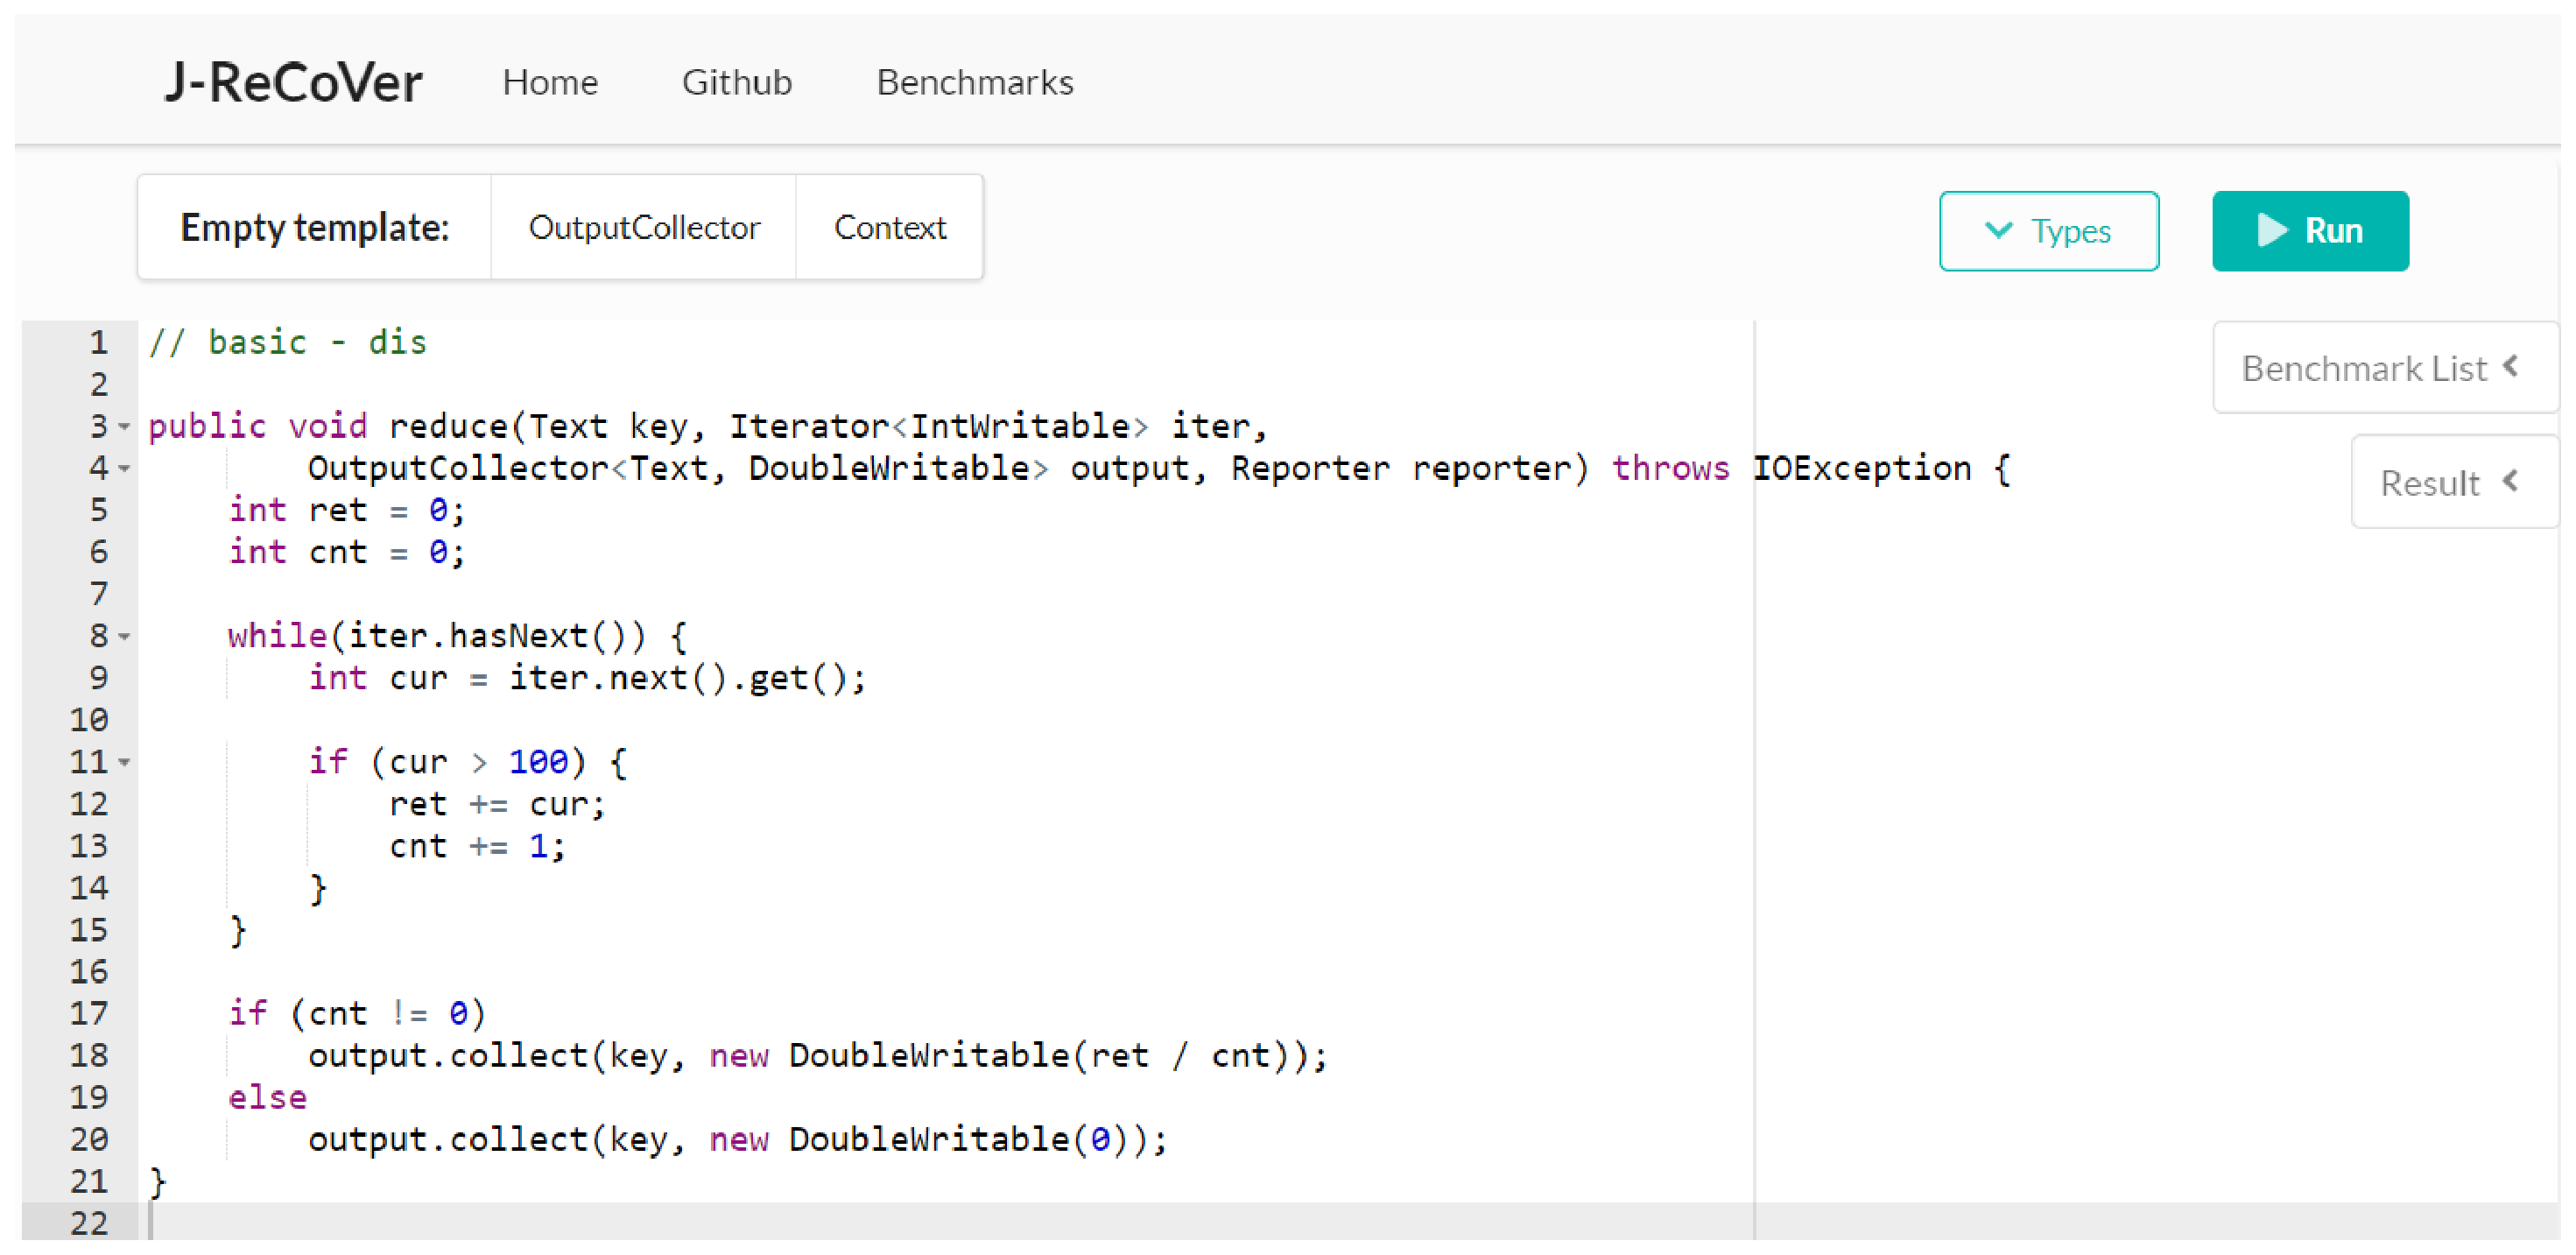
\includegraphics[width=.9\linewidth]{screenshots/main_screen.eps}
% \vspace{-5pt}
\caption{Main Screen of J-ReCoVer}
\label{fig:main_screen}
% \vspace{-15pt}
\end{center}
\end{figure}

\begin{itemize}
\item
Top Menu:
\begin{itemize}
\item
\emph{"Github"} opens a new tab of the repository of J-ReCoVer. The repository also has source code of benchmarks.
\item
\emph{"Benchmark"} leads to the list of benchmarks we collected with their results of commutativity analysis as Fig.~\ref{fig:benchmark_list} shows. Select the filename or "try it" button will select the example and go back to the main screen.
\end{itemize}
\item
Right Menu:
\begin{itemize}
\item
\emph{"Benchmark List"} provides a quick selection to examples in the benchmark (Fig.~\ref{fig:benchmark_list_right})
\item
\emph{"Results"} shows the last analysis result.
\end{itemize}
\item
Upper-Right Menu:
\begin{itemize}
\item
\emph{"Type"} provides types that J-ReCoVer supports. Details are explained in~\ref{appendix:3}.
\item
\emph{"Run"} starts the analysis of the selected example.
\end{itemize}
\item
Upper-Left Menu: See~\ref{appendix:3}.
\end{itemize}

\begin{figure}
\begin{center}
% \vspace{-10pt}
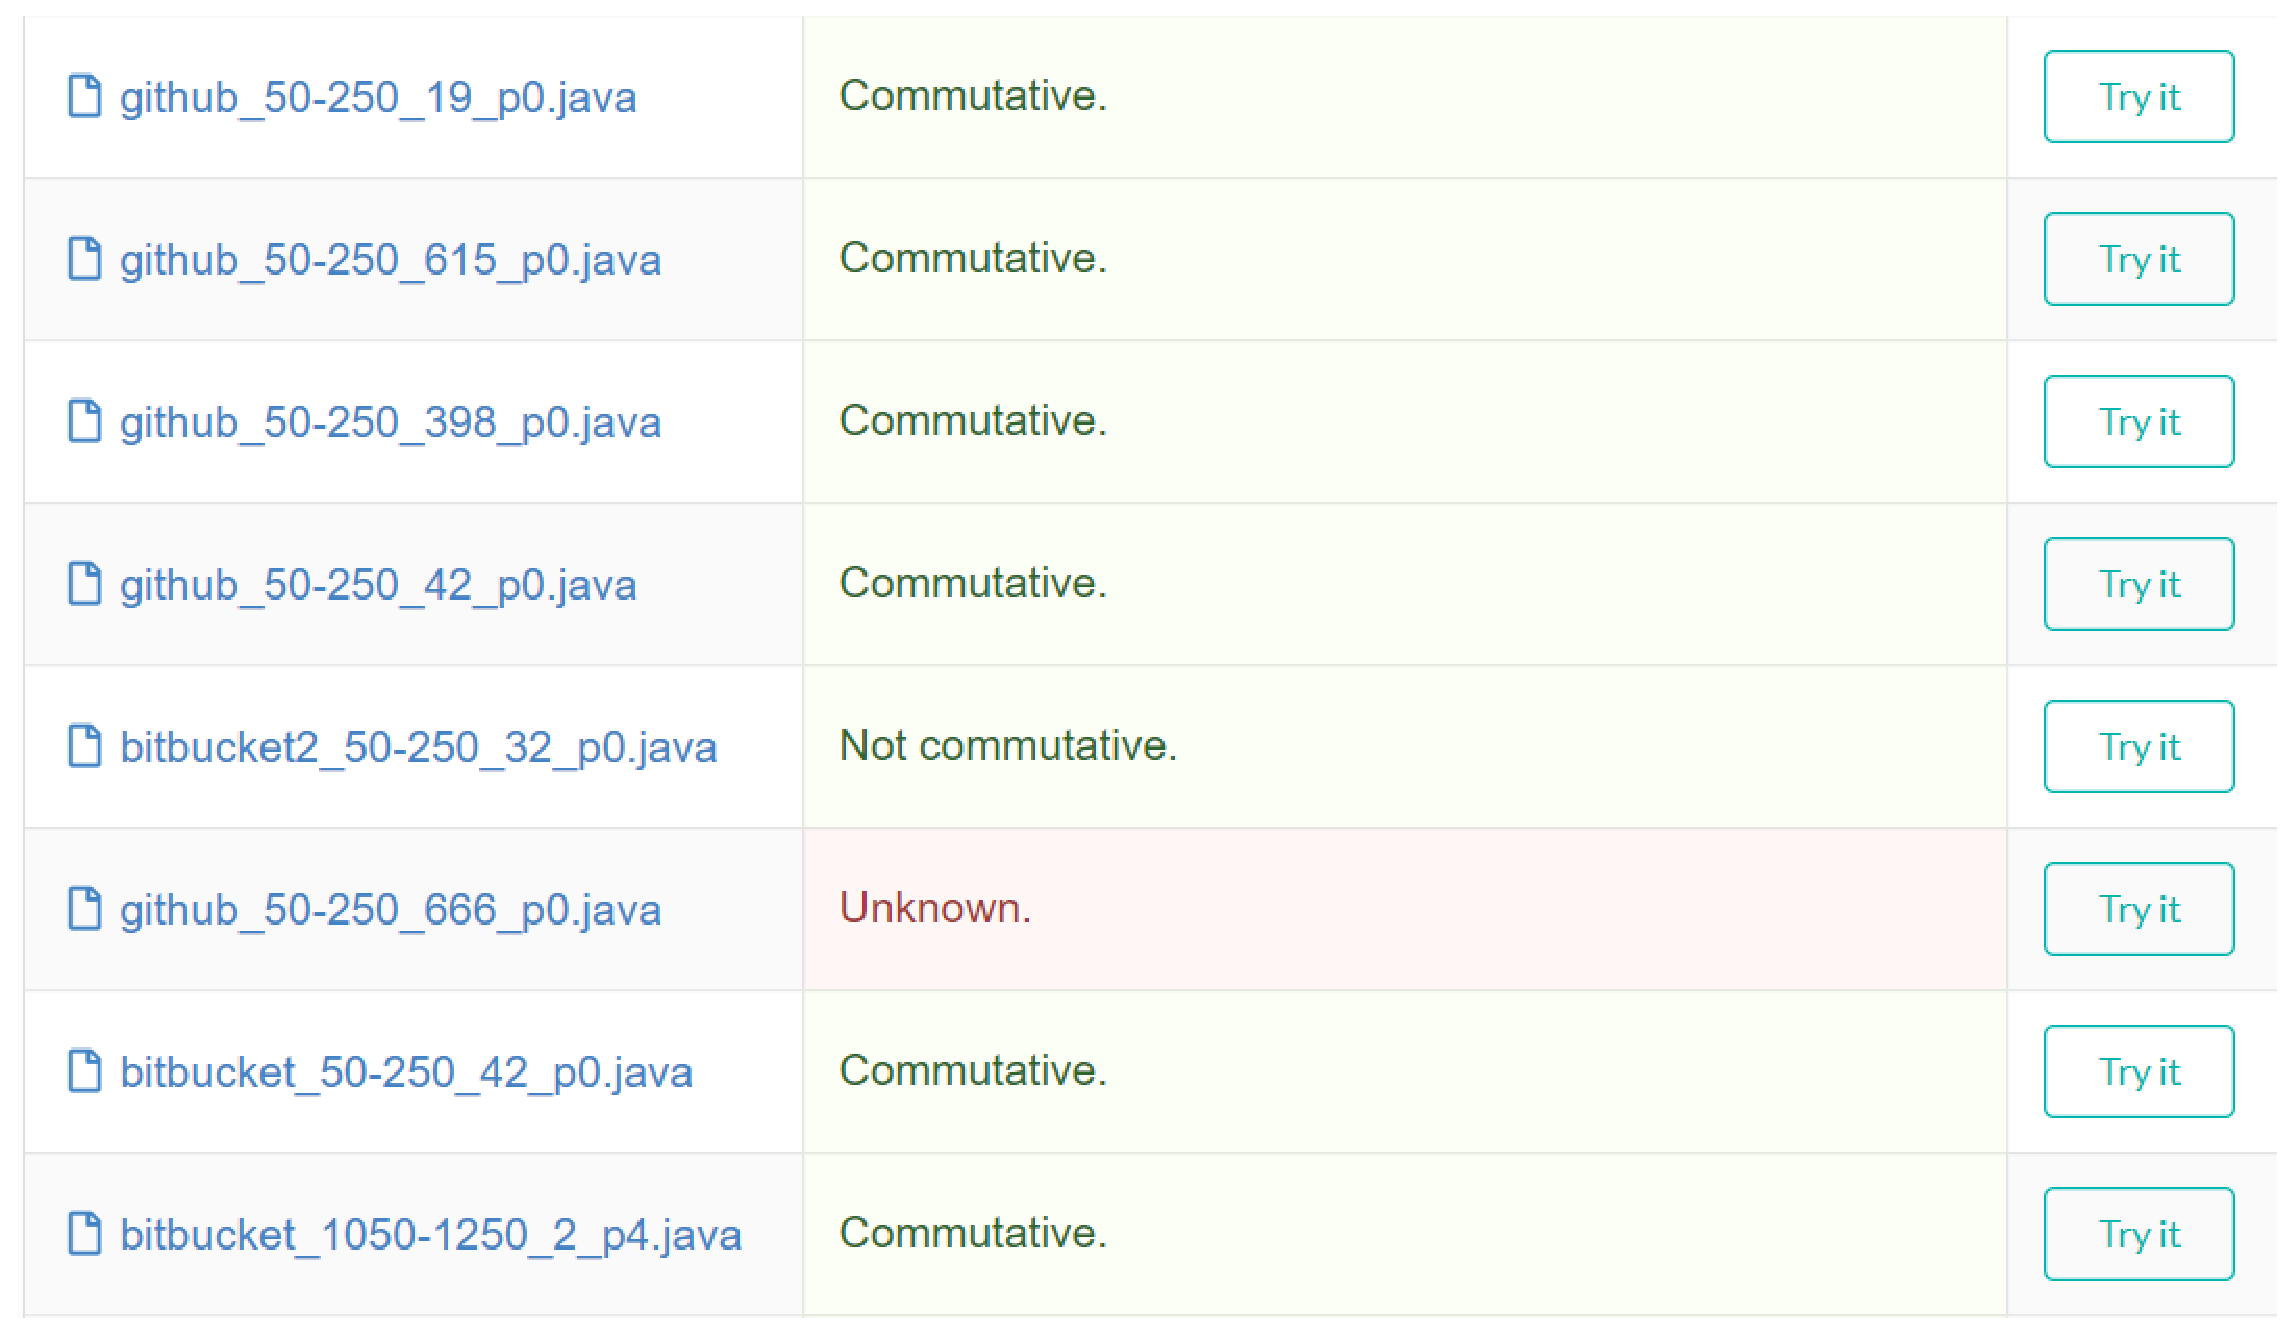
\includegraphics[width=.8\linewidth]{screenshots/benchmark_list.eps}
% \vspace{-5pt}
\caption{Benchmark list from top menu (part)}
\label{fig:benchmark_list}
% \vspace{-15pt}
\end{center}
\end{figure}

\begin{figure}
\begin{center}
% \vspace{-10pt}
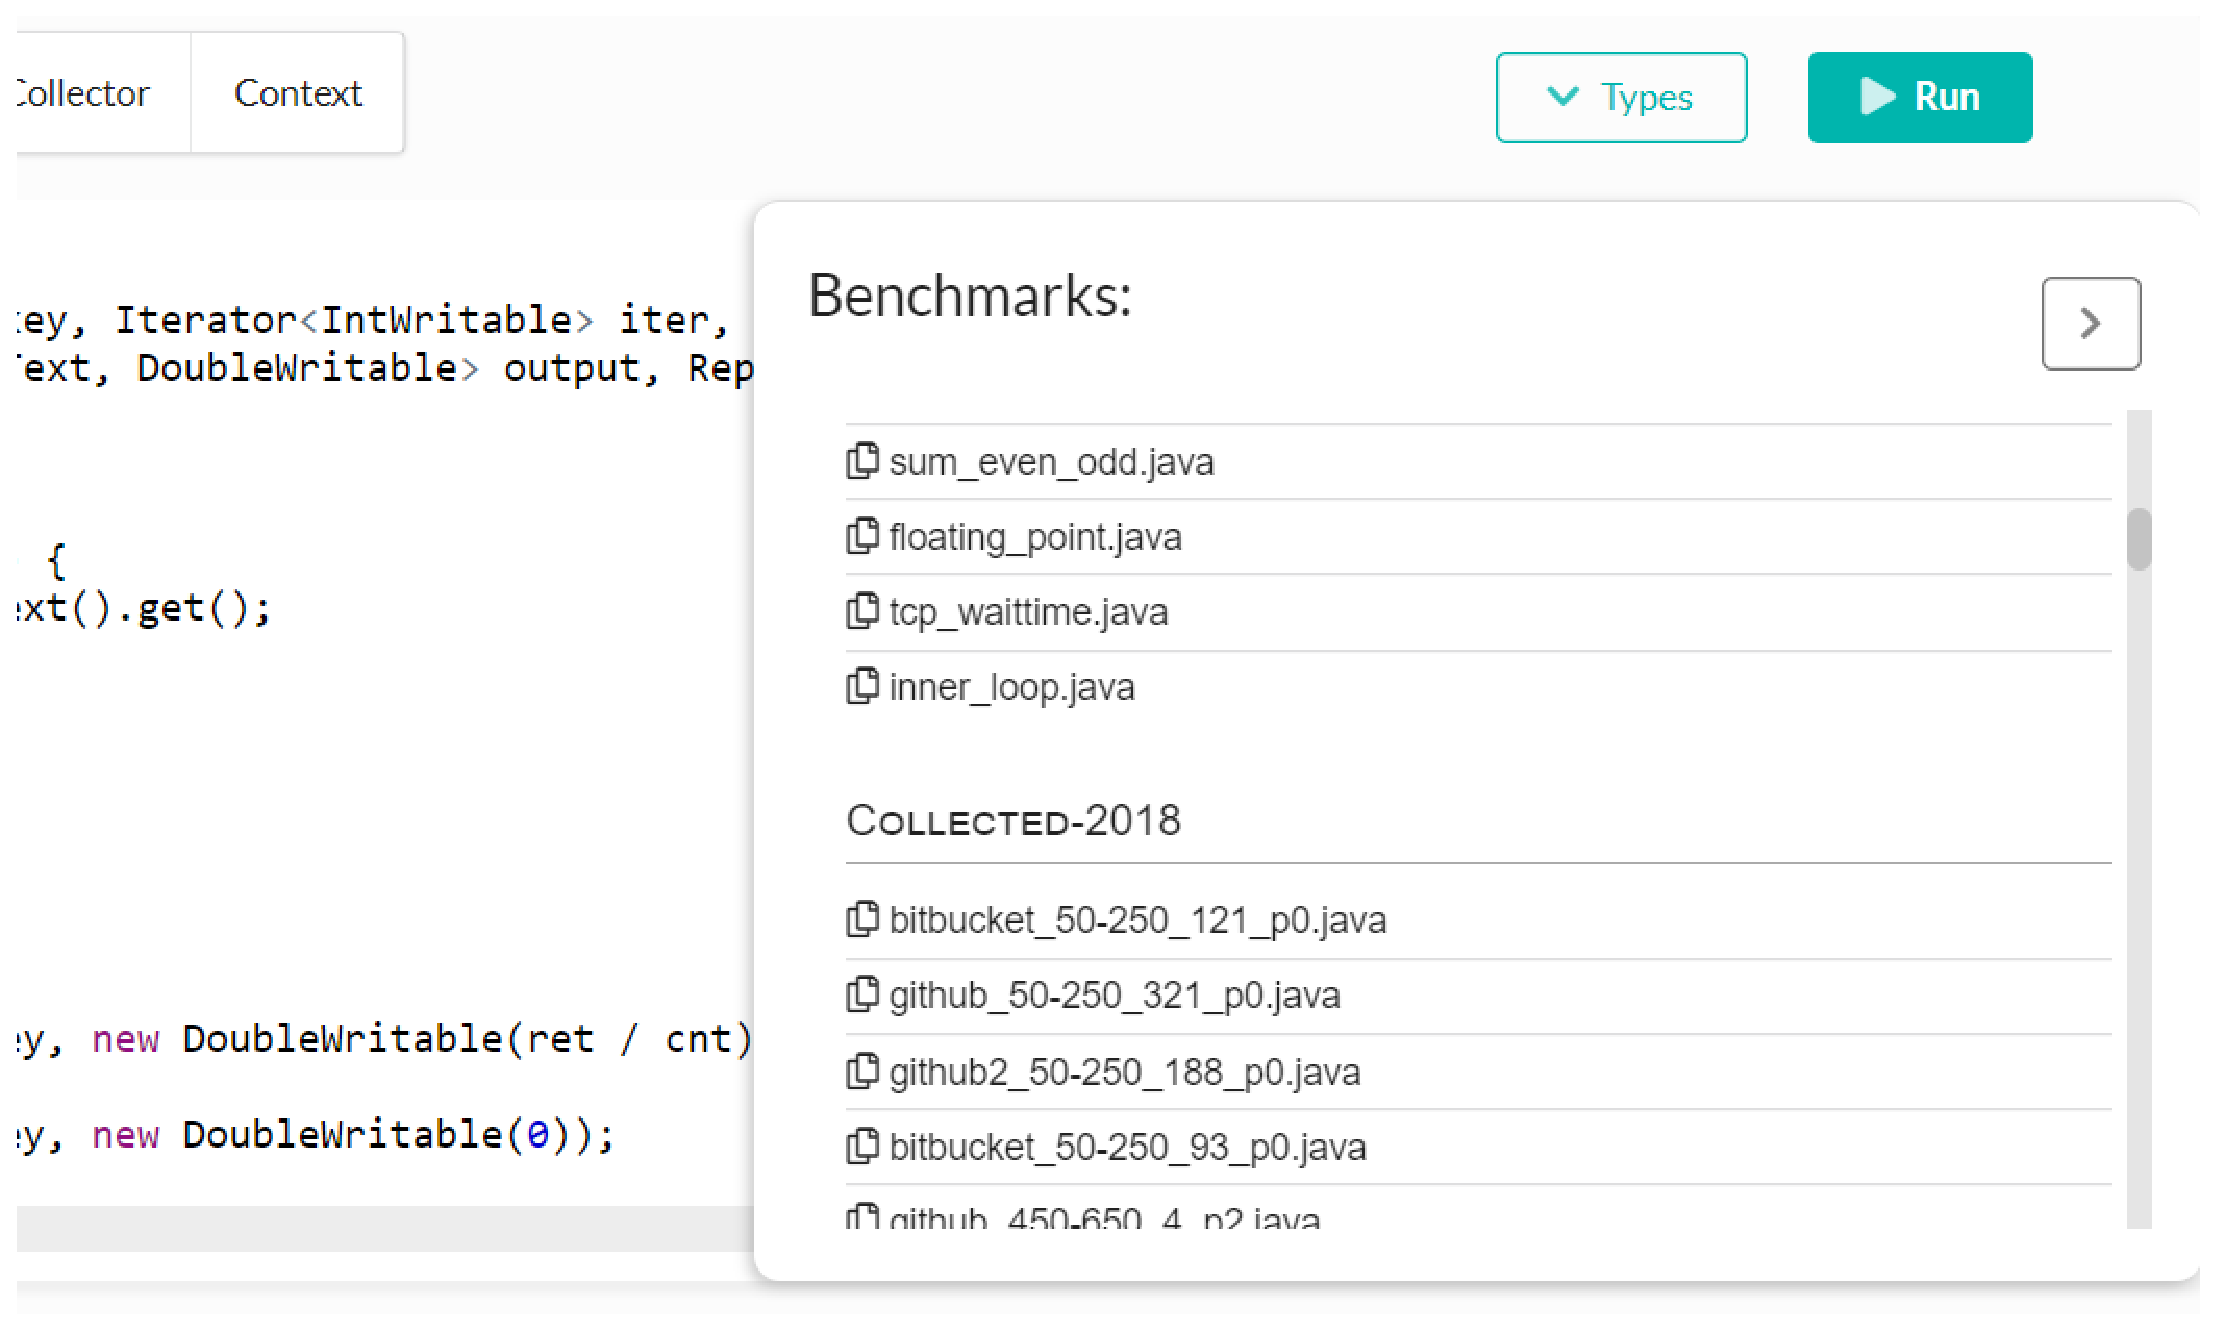
\includegraphics[width=.8\linewidth]{screenshots/benchmark_list_right.eps}
% \vspace{-5pt}
\caption{Benchmark list from right menu (part)}
\label{fig:benchmark_list_right}
% \vspace{-15pt}
\end{center}
\end{figure}

\subsection{Run analysis of selected benchmark example}
\label{appendix:2}

To run analysis, you can choose an example from benchmark using either the top menu or the right menu, then click the "Run" button of the upper-right menu to start the commutativity analysis of the selected example. The pull-down menu "Types" of the upper-right menu provides selectable types for input \texttt{(T1,T2)} and output \texttt{(T3,T4)}. Fig.~\ref{fig:type_select_menu} shows the pull-down menu and Fig.~\ref{fig:selectable_types} shows part of the selectable types in J-ReCoVer. If one selects an example from the benchmark, the types will be automatically selected to match the example. The selection will be needed if the user wants to write a reduce function from sketch for analysis (see~\ref{appendix:3}).

\begin{figure}
\begin{center}
% \vspace{-10pt}
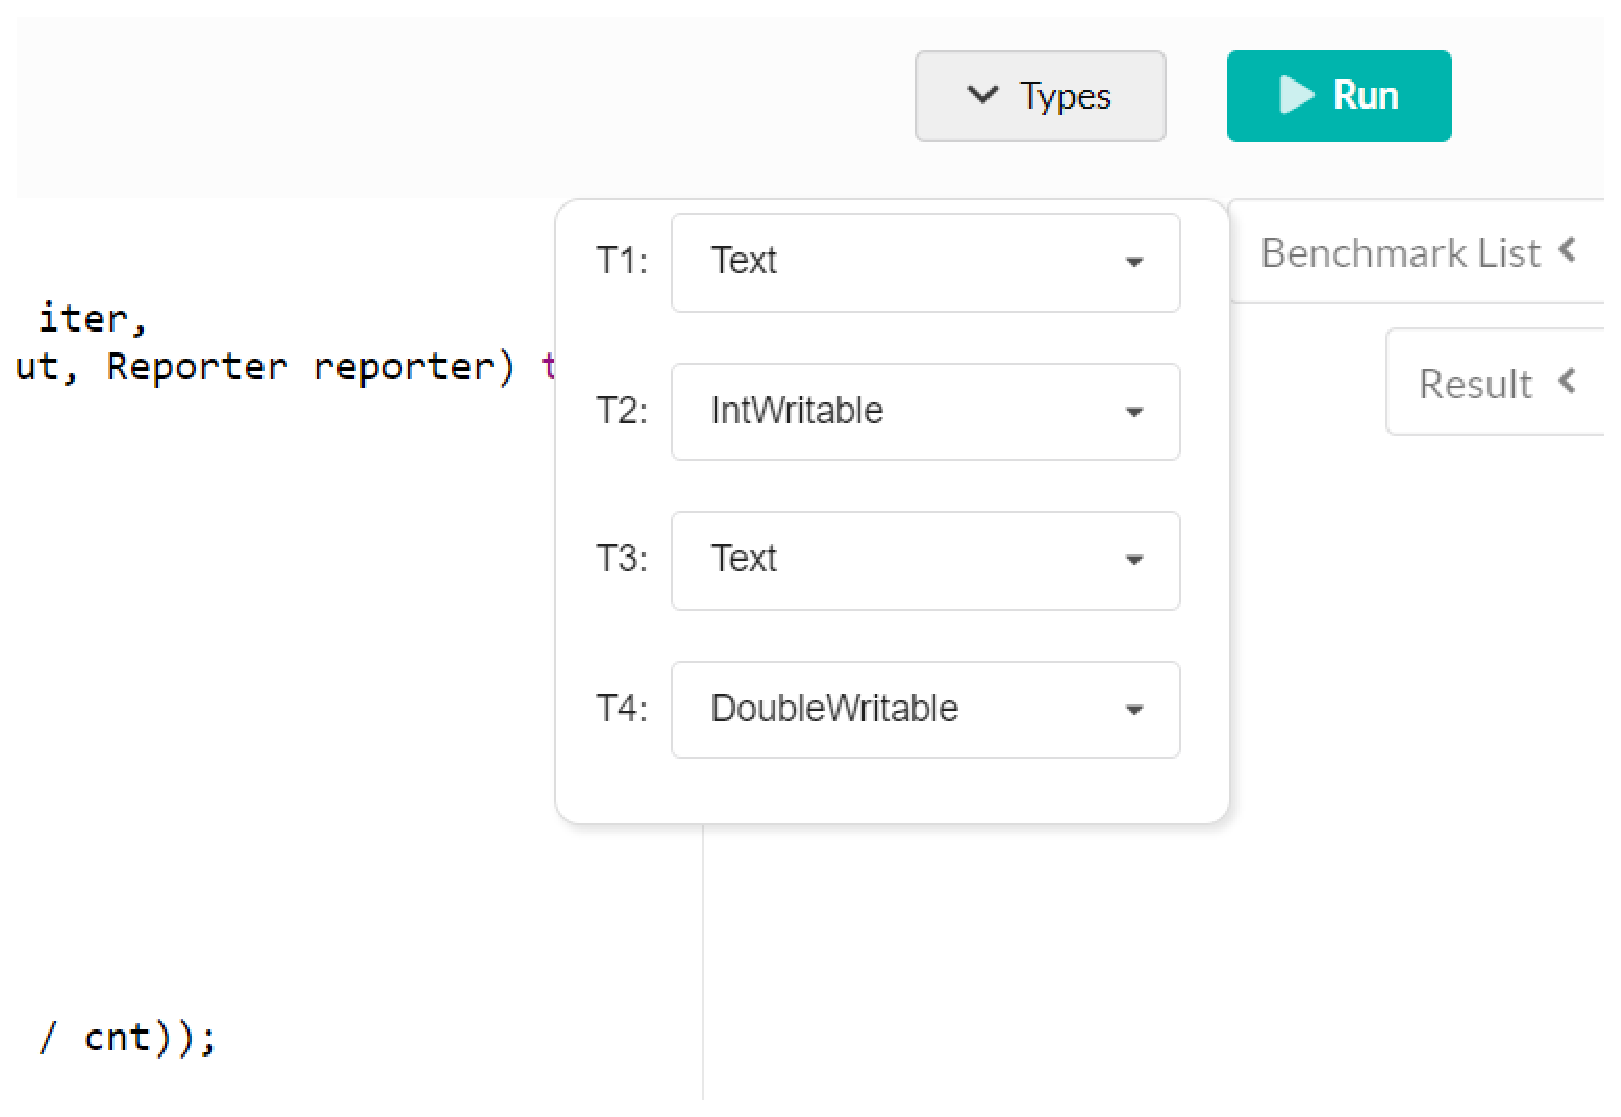
\includegraphics[width=.8\linewidth]{screenshots/type_select_menu.eps}
% \vspace{-5pt}
\caption{Type select menu}
\label{fig:type_select_menu}
% \vspace{-15pt}
\end{center}
\end{figure}

\begin{figure}
\begin{center}
% \vspace{-10pt}
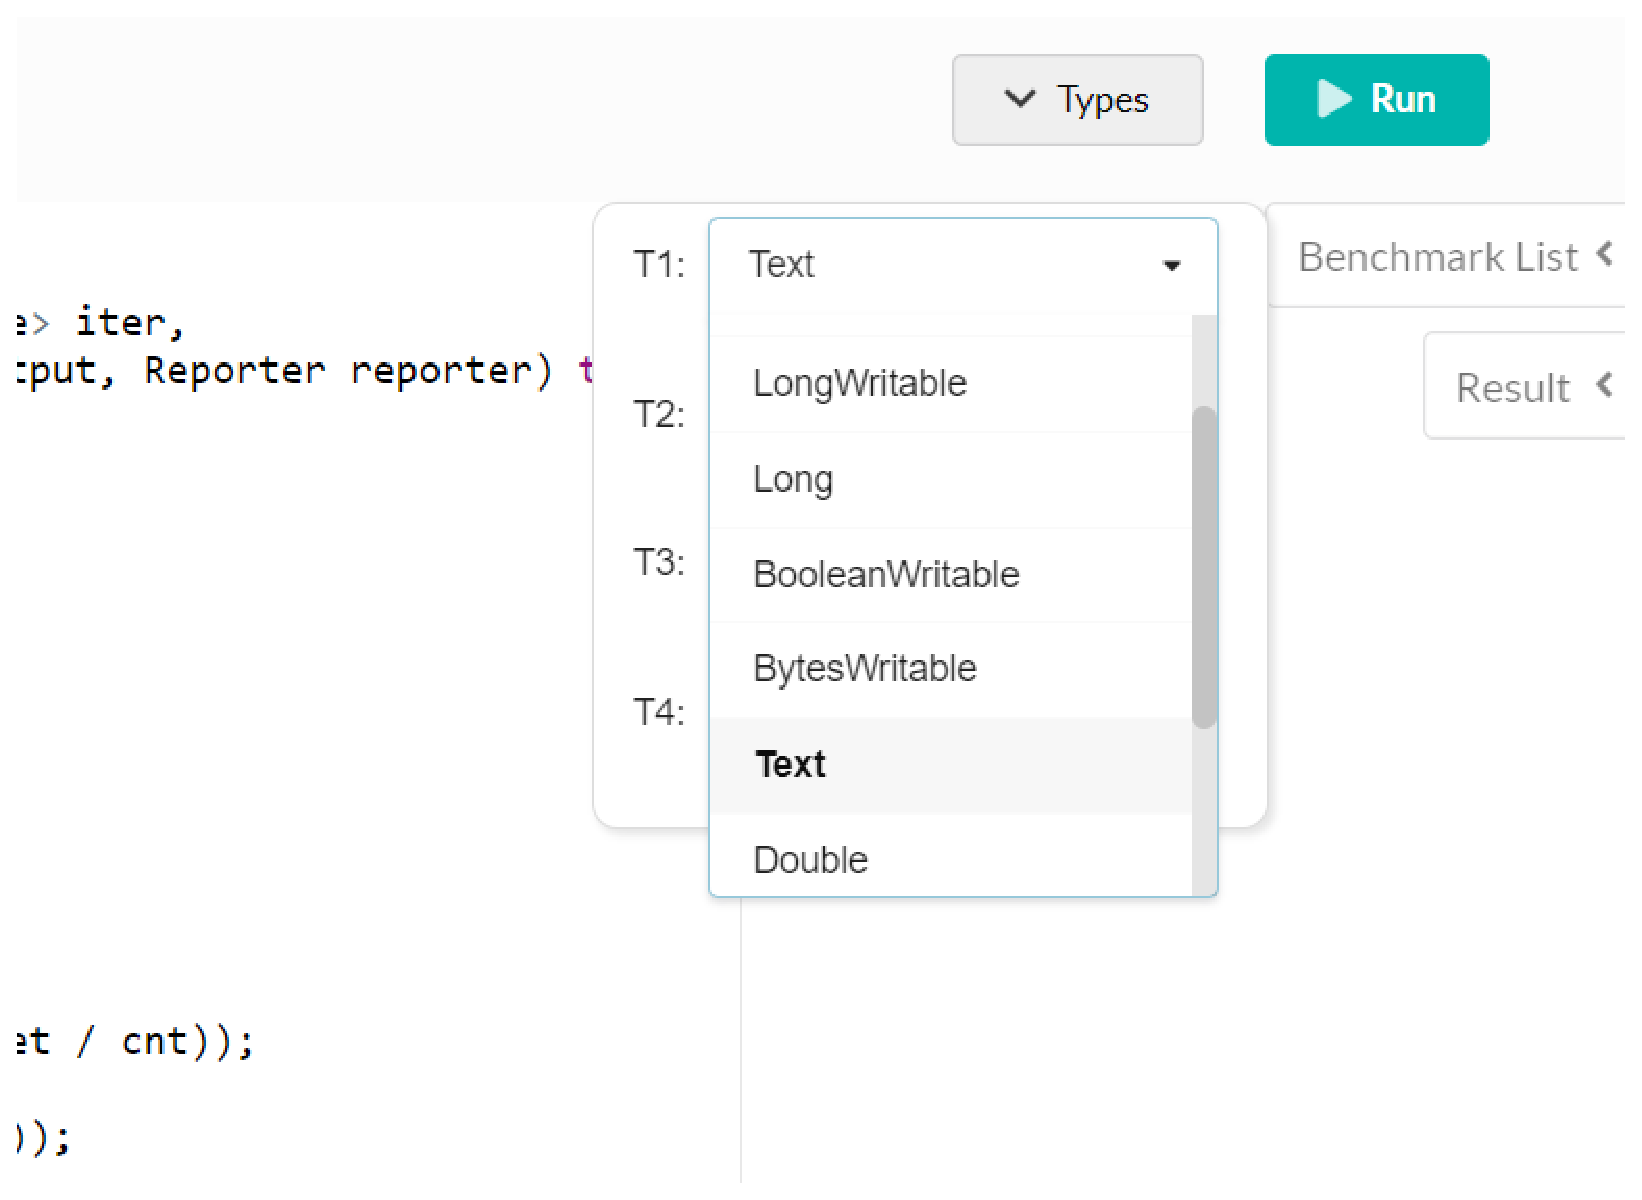
\includegraphics[width=.8\linewidth]{screenshots/selectable_types.eps}
% \vspace{-5pt}
\caption{Selectable types (part)}
\label{fig:selectable_types}
% \vspace{-15pt}
\end{center}
\end{figure}

After J-ReCoVer finishes the analysis, the \emph{"Result:"} tab of the right menu will show the result as Fig.~\ref{fig:analysis_result} shows. Fig.~\ref{fig:analysis_result_text} shows the analysis result of the first benchmark \texttt{dis.java} in detail.

\begin{figure}
\begin{center}
% \vspace{-10pt}
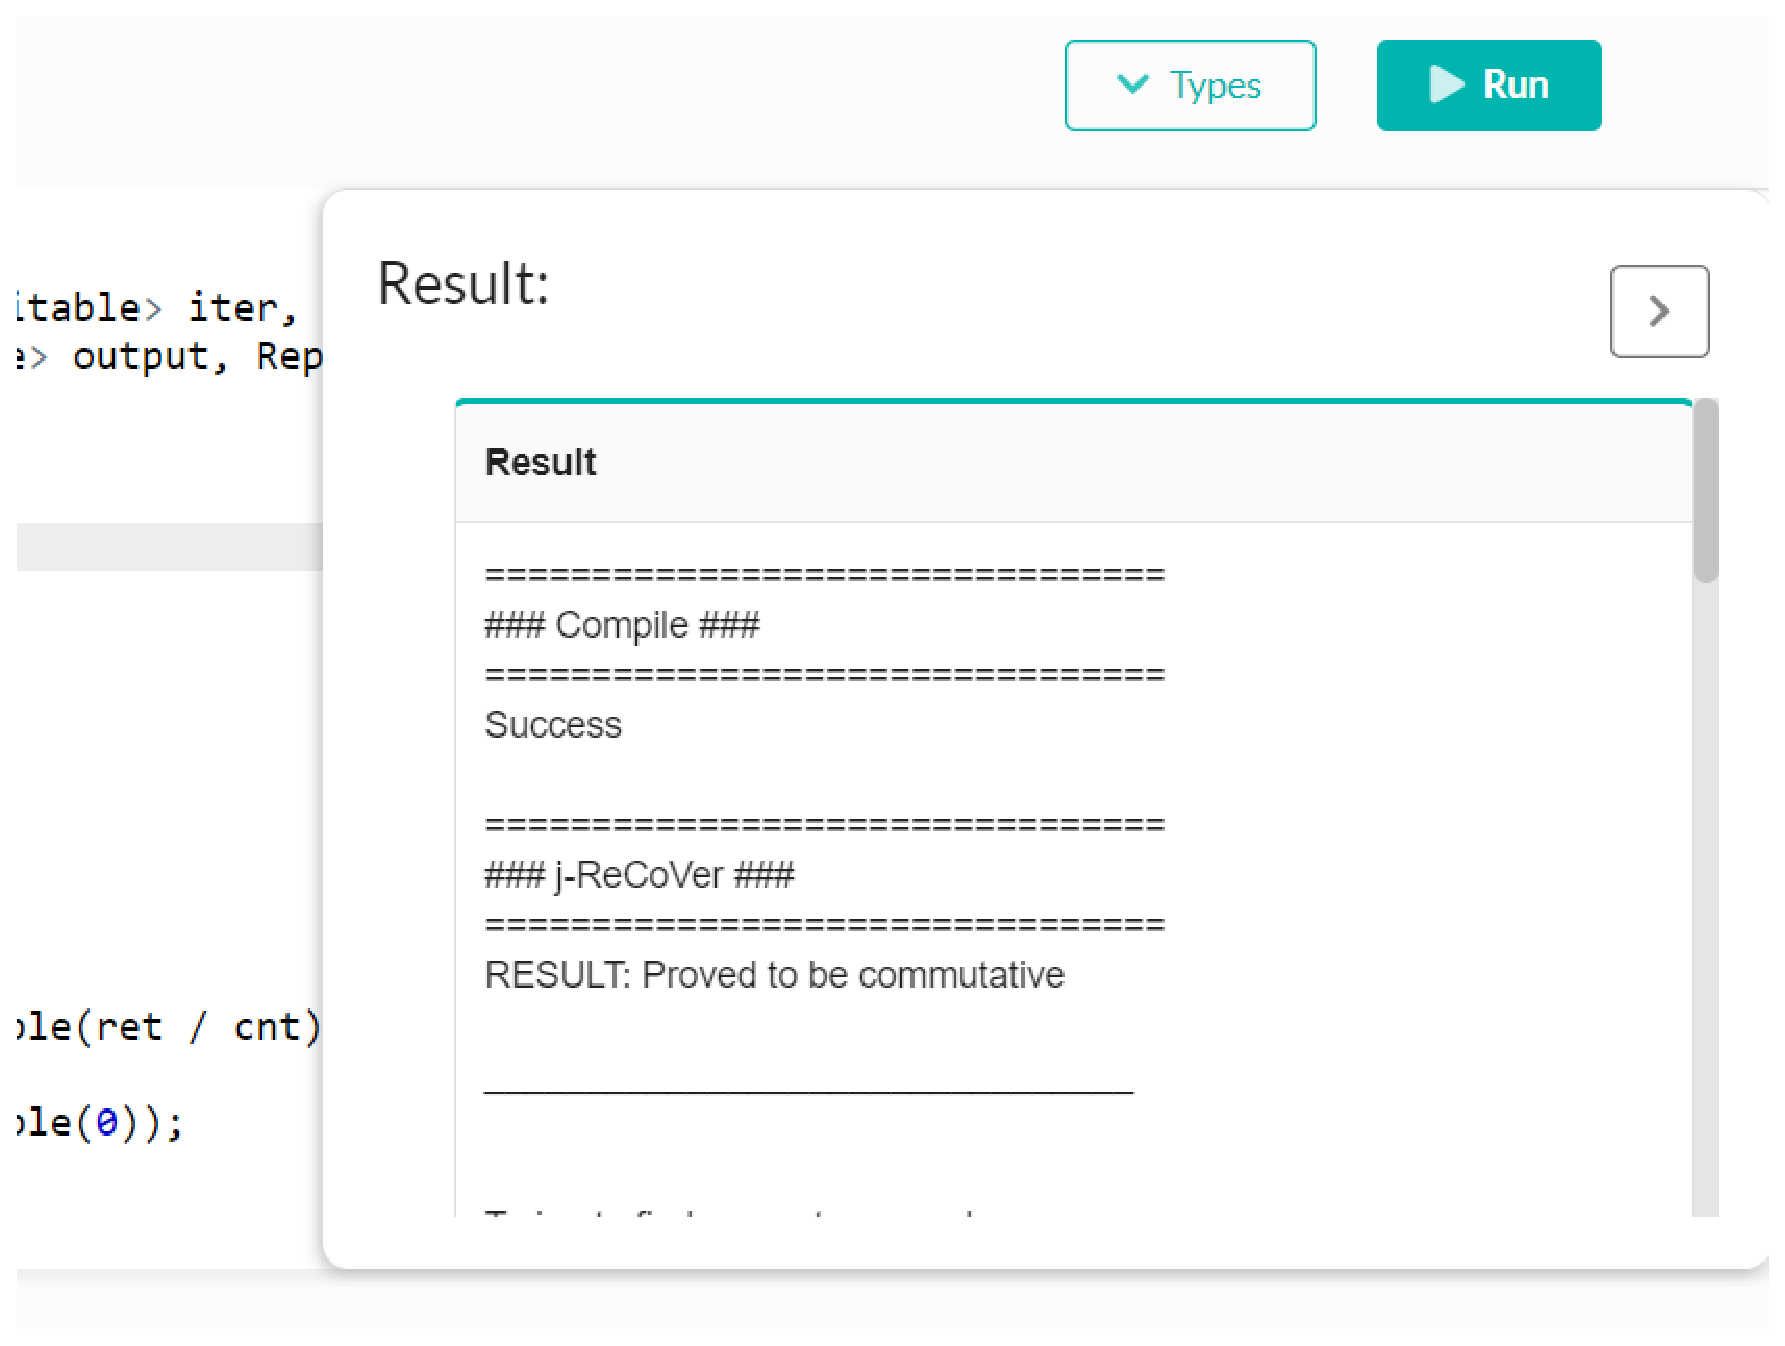
\includegraphics[width=.8\linewidth]{screenshots/analysis_result.eps}
% \vspace{-5pt}
\caption{The analysis result}
\label{fig:analysis_result}
% \vspace{-15pt}
\end{center}
\end{figure}

\begin{figure}
\begin{center}
\begin{mdframed}[roundcorner=5pt]
\begin{Verbatim}[fontsize=\tiny]
================================
### Compile ###
================================
Success

================================
### j-ReCoVer ###
================================
RESULT: Proved to be commutative

________________________________


Trying to find a counterexample...

RESULT: Cannot find a counterexample in 500 tests
Testcases were generated randomly.

Following are the first 50 lines of testcases:
Input1: o [5, 4, 5, 2, -1]
Input2: o [-1, 4, 5, 5, 2]
Output1: 

Key: [o]
Val: [0.0]
--
Output2: 

Key: [o]
Val: [0.0]
--------
Input1: j [1, -1, 0, 3, -2]
Input2: j [0, 3, -2, 1, -1]
Output1: 

Key: [j]
Val: [0.0]
--
Output2: 

Key: [j]
Val: [0.0]
--------
Input1: e [4, 3, 5, -4, 1]
Input2: e [4, -4, 5, 3, 1]
Output1: 

Key: [e]
Val: [0.0]
--
Output2: 

Key: [e]
Val: [0.0]
--------
Input1: s [3, 0, 2, -4, -1]
Input2: s [3, -1, 0, -4, 2]
Output1: 

Key: [s]
Val: [0.0]
--
Output2: 

Key: [s]
Val: [0.0]
--------
Input1: v [-3, -2, 3, 3, -3]
Input2: v [3, -2, -3, -3, 3]
\end{Verbatim}
\end{mdframed}
\caption{The analysis result of \texttt{dis.java}}
\label{fig:analysis_result_text}
\end{center}
\end{figure}

In a commutativity analysis, J-ReCoVer first tries to compile the example then perfrom commutativity analysis. If the analysis says the example is commutative, J-ReCoVer then runs 500 randomly generated test cases to try to find a counterexample. If the test cases all pass, J-ReCoVer concludes that the example is commutative, or the result will be "unknown" since the results of analysis and tests are inconsistent. For the case that the commutativity analysis returns false, J-ReCoVer will also run test cases to find a counterexample. This time, J-ReCoVer will conclude "not commutative" if a counterexample is found, or "unknown" if no counterexample is found. 

\subsection{Run Analysis of an example from sketch}
\label{appendix:3}

Besides examples from the benchmark, J-ReCoVer also provides an interactive way to analyze a reduce function starting from a sketch.
The upper-left menu (below the top menu) provides blank templates for two versions of Hadoop. The templates are

\begin{mdframed}[roundcorner=5pt]
\begin{verbatim}
public void reduce(T1 key, Iterator<T2> values,
	OutputCollector<T3,T4> oc1, Reporter reporter)
		throws IOException,InterruptedException {

}
\end{verbatim}
\end{mdframed}

, and

\begin{mdframed}[roundcorner=5pt]
\begin{verbatim}
public void reduce(T1 key, Iterable<T2> values,
	Context context) throws IOException,InterruptedException {

}
\end{verbatim}
\end{mdframed}

In this case, one would have to manually fill the types T1 to T4 and the function body, then selects the types from the pull-down menu, as shown in Fig.~\ref{fig:type_select_menu} and Fig.~\ref{fig:selectable_types}.

For more details, all selectable types are:

\begin{itemize}
\item Long
\item BooleanWritable
\item BytesWritable
\item Text
\item Double
\item DoubleWritable
\item Float
\item FloatWritable
\end{itemize}

\clearpage
\appendix

\section{J-ReCoVer Usages}

\subsection{The User Interface of J-ReCoVer}
\label{appendix:1}

J-ReCoVer is available online at \url{\texttt{http://jrecover.iis.sinica.edu.tw/}}. Fig.~\ref{fig:main_screen} shows the main screen of J-ReCoVer. The alignment of user interface elements are as follows:

\begin{figure}
\begin{center}
% \vspace{-10pt}
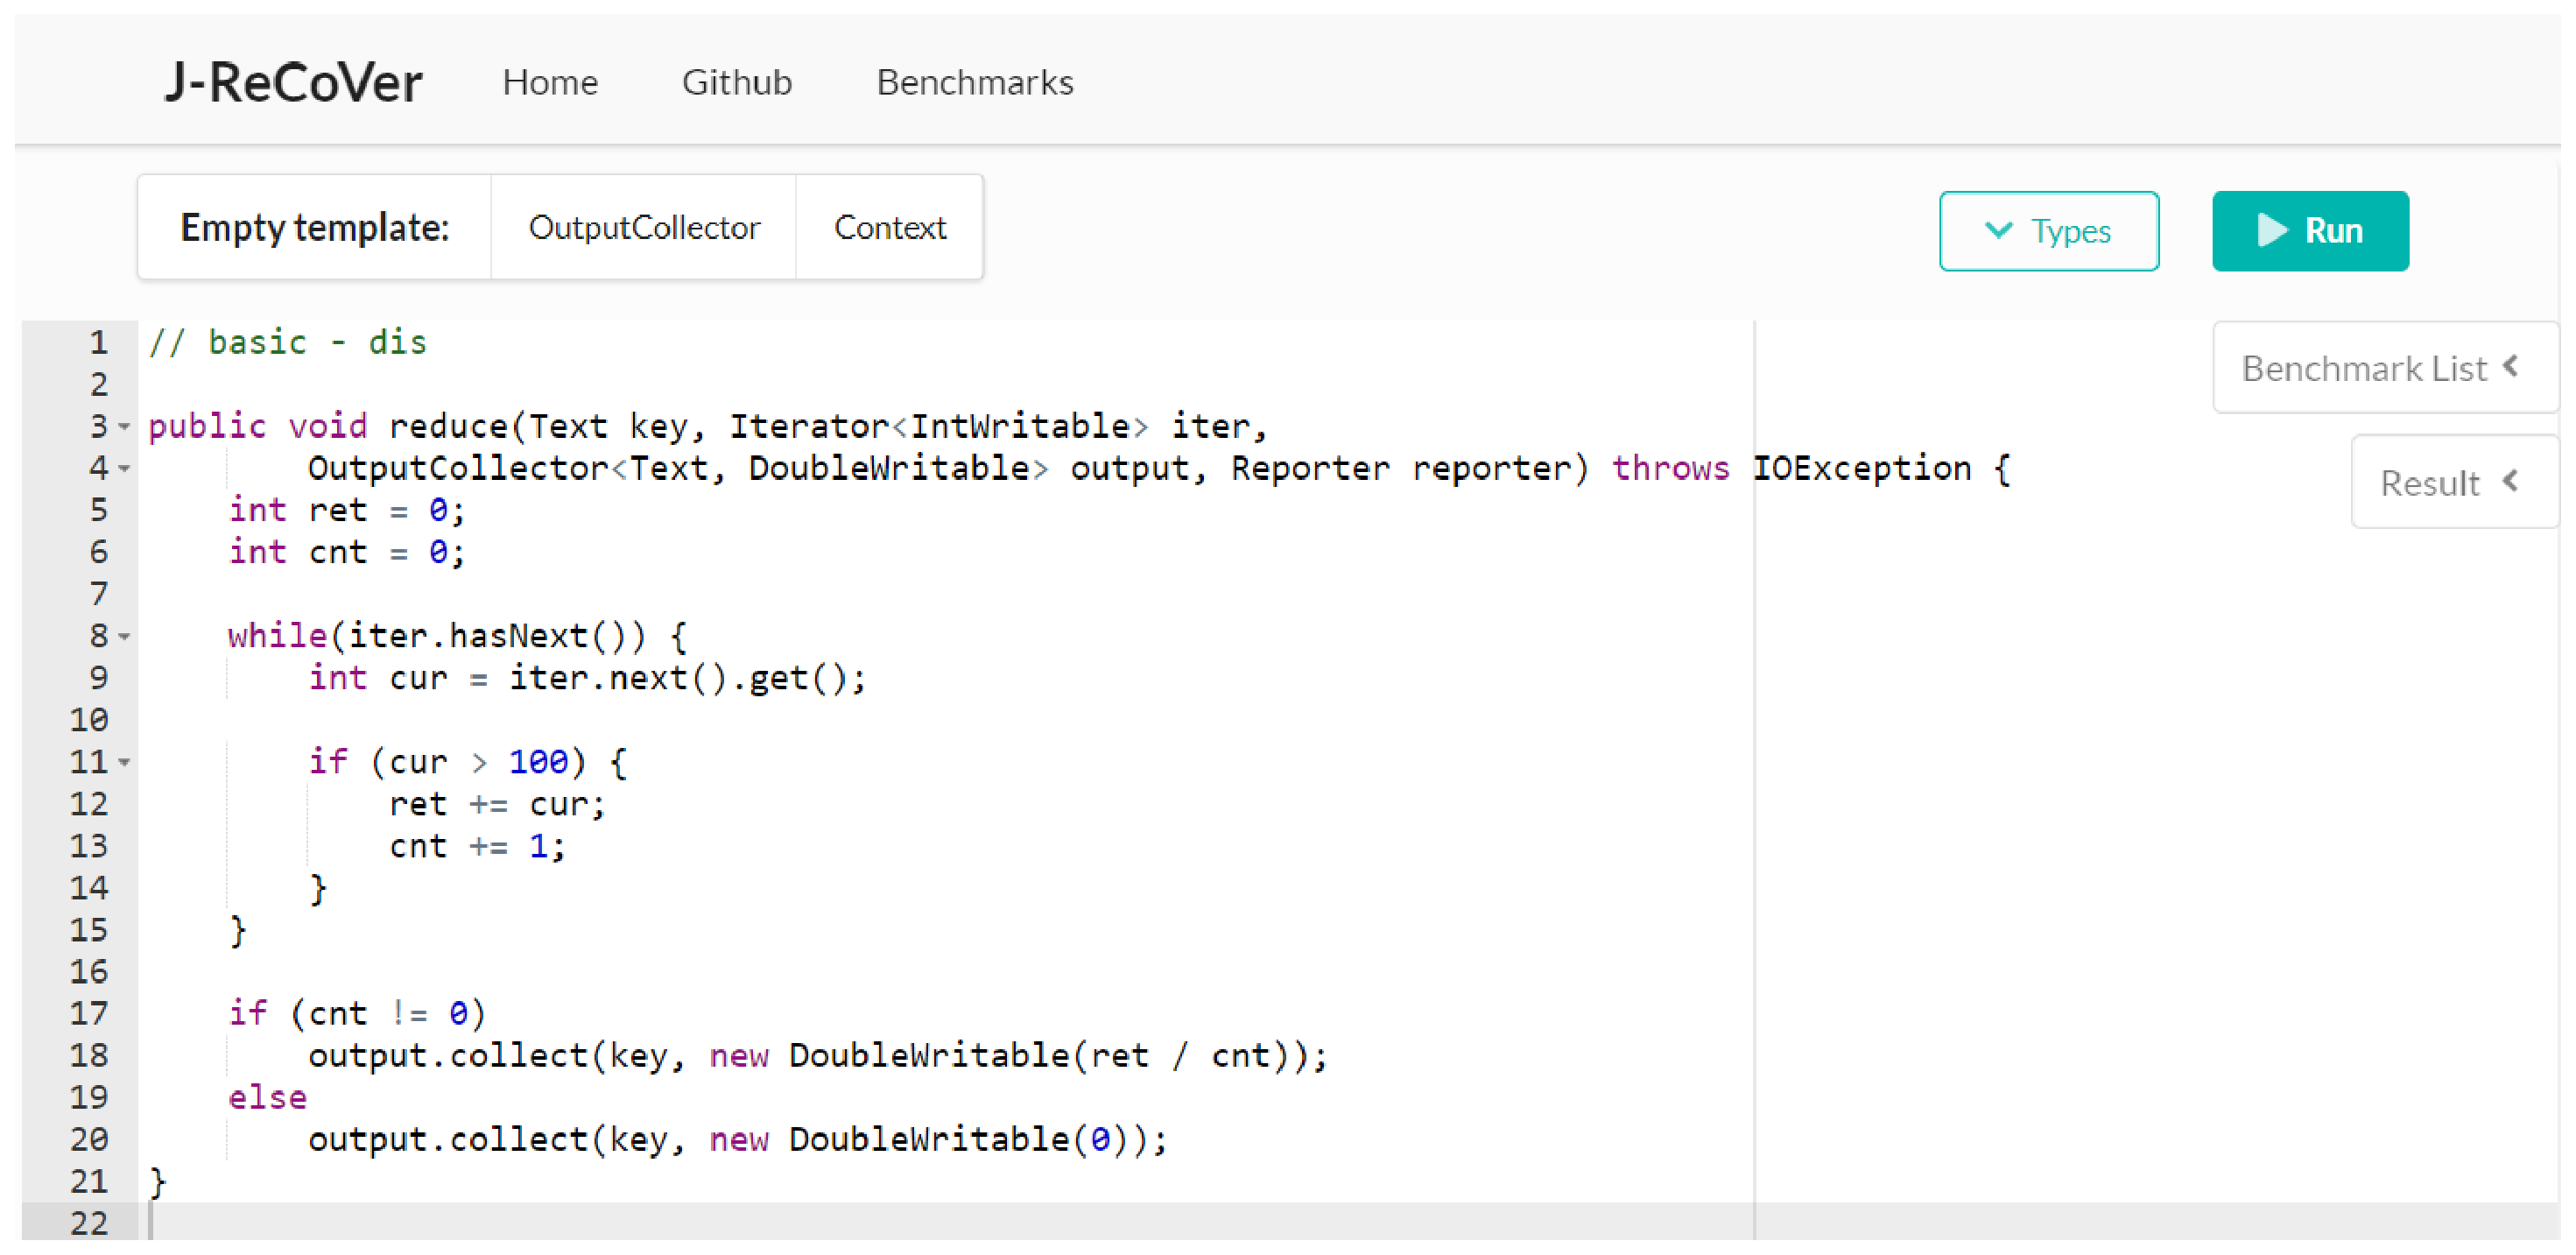
\includegraphics[width=.9\linewidth]{screenshots/main_screen.eps}
% \vspace{-5pt}
\caption{Main Screen of J-ReCoVer}
\label{fig:main_screen}
% \vspace{-15pt}
\end{center}
\end{figure}

\begin{itemize}
\item
Top Menu:
\begin{itemize}
\item
\emph{"Github"} opens a new tab of the repository of J-ReCoVer. The repository also has source code of benchmarks.
\item
\emph{"Benchmark"} leads to the list of benchmarks we collected with their results of commutativity analysis as Fig.~\ref{fig:benchmark_list} shows. Select the filename or "try it" button will select the example and go back to the main screen.
\end{itemize}
\item
Right Menu:
\begin{itemize}
\item
\emph{"Benchmark List"} provides a quick selection to examples in the benchmark (Fig.~\ref{fig:benchmark_list_right})
\item
\emph{"Results"} shows the last analysis result.
\end{itemize}
\item
Upper-Right Menu:
\begin{itemize}
\item
\emph{"Type"} provides types that J-ReCoVer supports. Details are explained in~\ref{appendix:3}.
\item
\emph{"Run"} starts the analysis of the selected example.
\end{itemize}
\item
Upper-Left Menu: See~\ref{appendix:3}.
\end{itemize}

\begin{figure}
\begin{center}
% \vspace{-10pt}
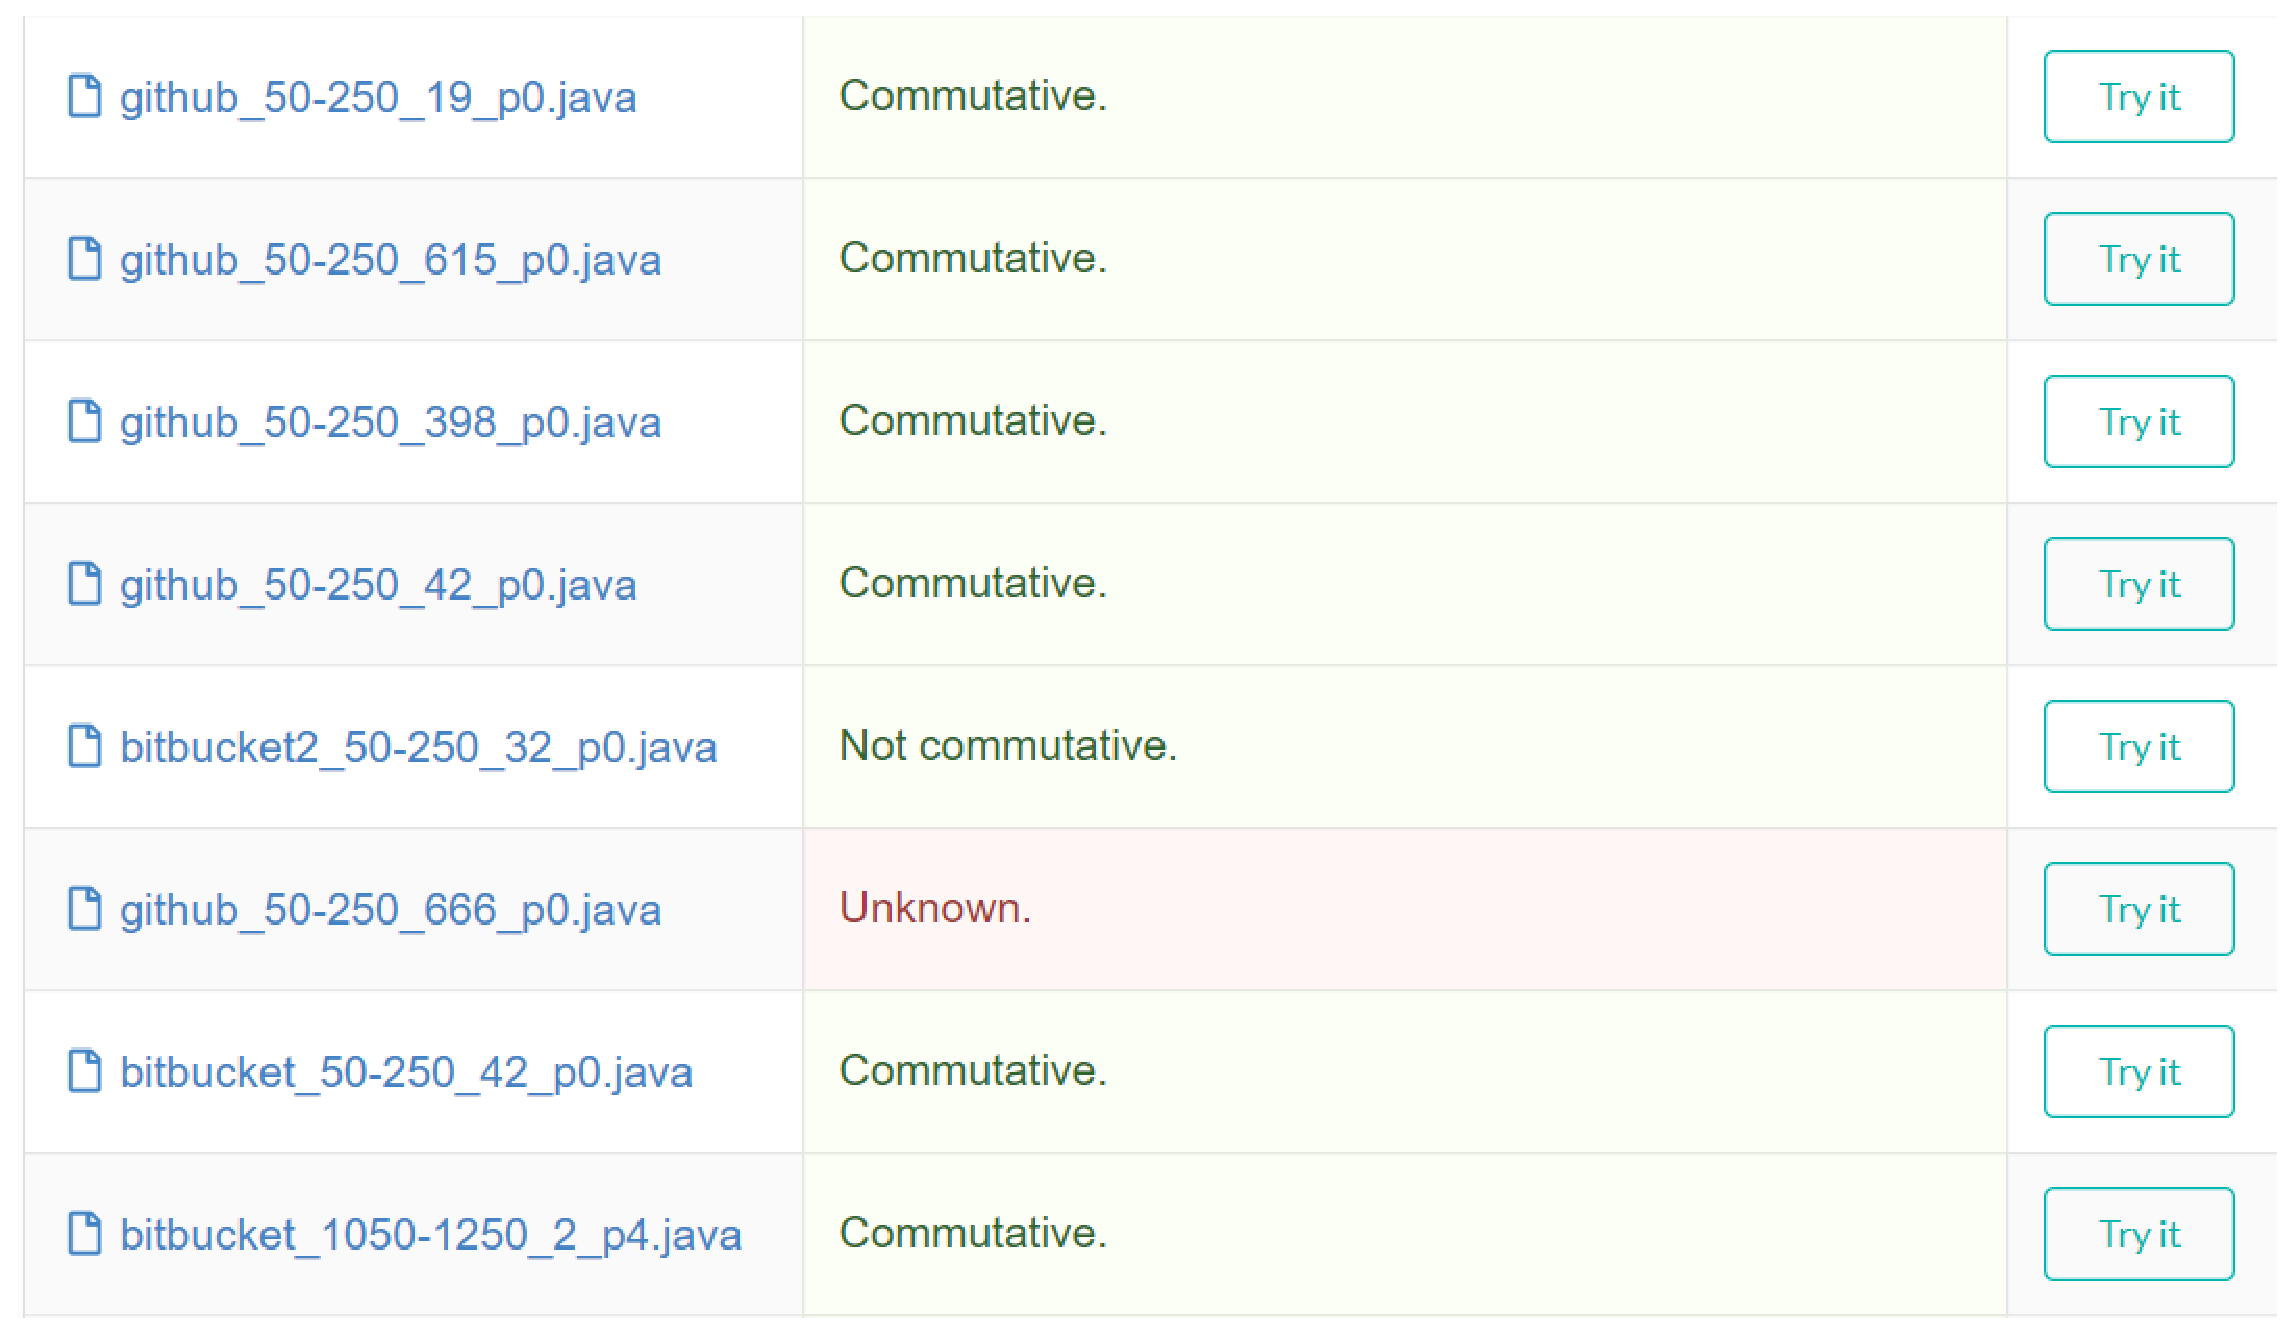
\includegraphics[width=.8\linewidth]{screenshots/benchmark_list.eps}
% \vspace{-5pt}
\caption{Benchmark list from top menu (part)}
\label{fig:benchmark_list}
% \vspace{-15pt}
\end{center}
\end{figure}

\begin{figure}
\begin{center}
% \vspace{-10pt}
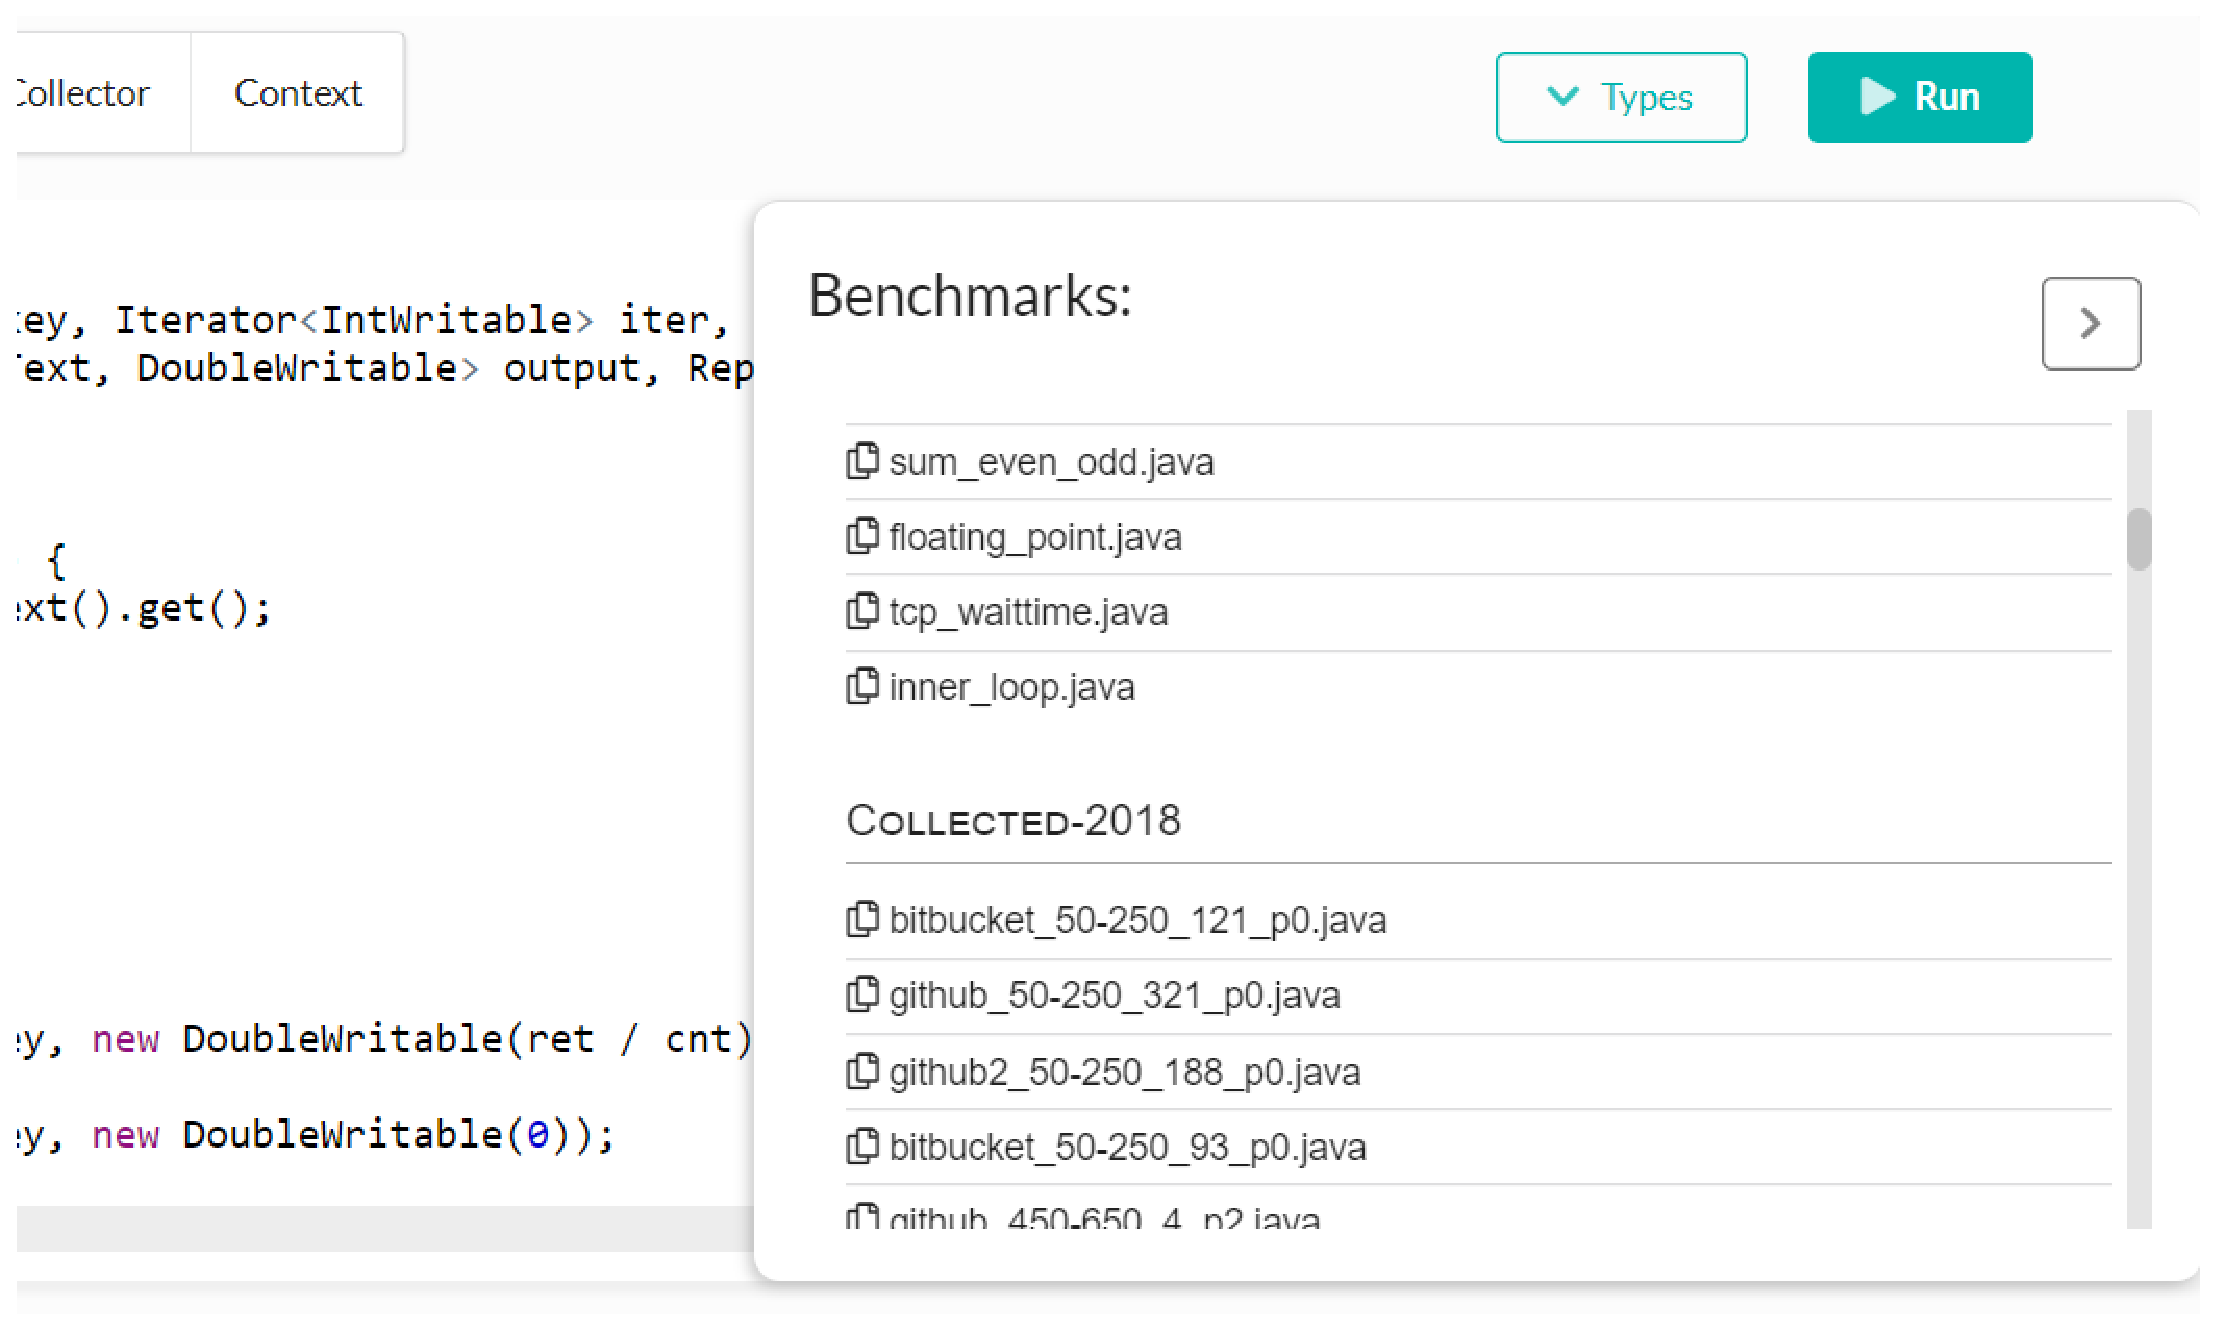
\includegraphics[width=.8\linewidth]{screenshots/benchmark_list_right.eps}
% \vspace{-5pt}
\caption{Benchmark list from right menu (part)}
\label{fig:benchmark_list_right}
% \vspace{-15pt}
\end{center}
\end{figure}

\subsection{Run analysis of selected benchmark example}
\label{appendix:2}

To run analysis, you can choose an example from benchmark using either the top menu or the right menu, then click the "Run" button of the upper-right menu to start the commutativity analysis of the selected example. The pull-down menu "Types" of the upper-right menu provides selectable types for input \texttt{(T1,T2)} and output \texttt{(T3,T4)}. Fig.~\ref{fig:type_select_menu} shows the pull-down menu and Fig.~\ref{fig:selectable_types} shows part of the selectable types in J-ReCoVer. If one selects an example from the benchmark, the types will be automatically selected to match the example. The selection will be needed if the user wants to write a reduce function from sketch for analysis (see~\ref{appendix:3}).

\begin{figure}
\begin{center}
% \vspace{-10pt}
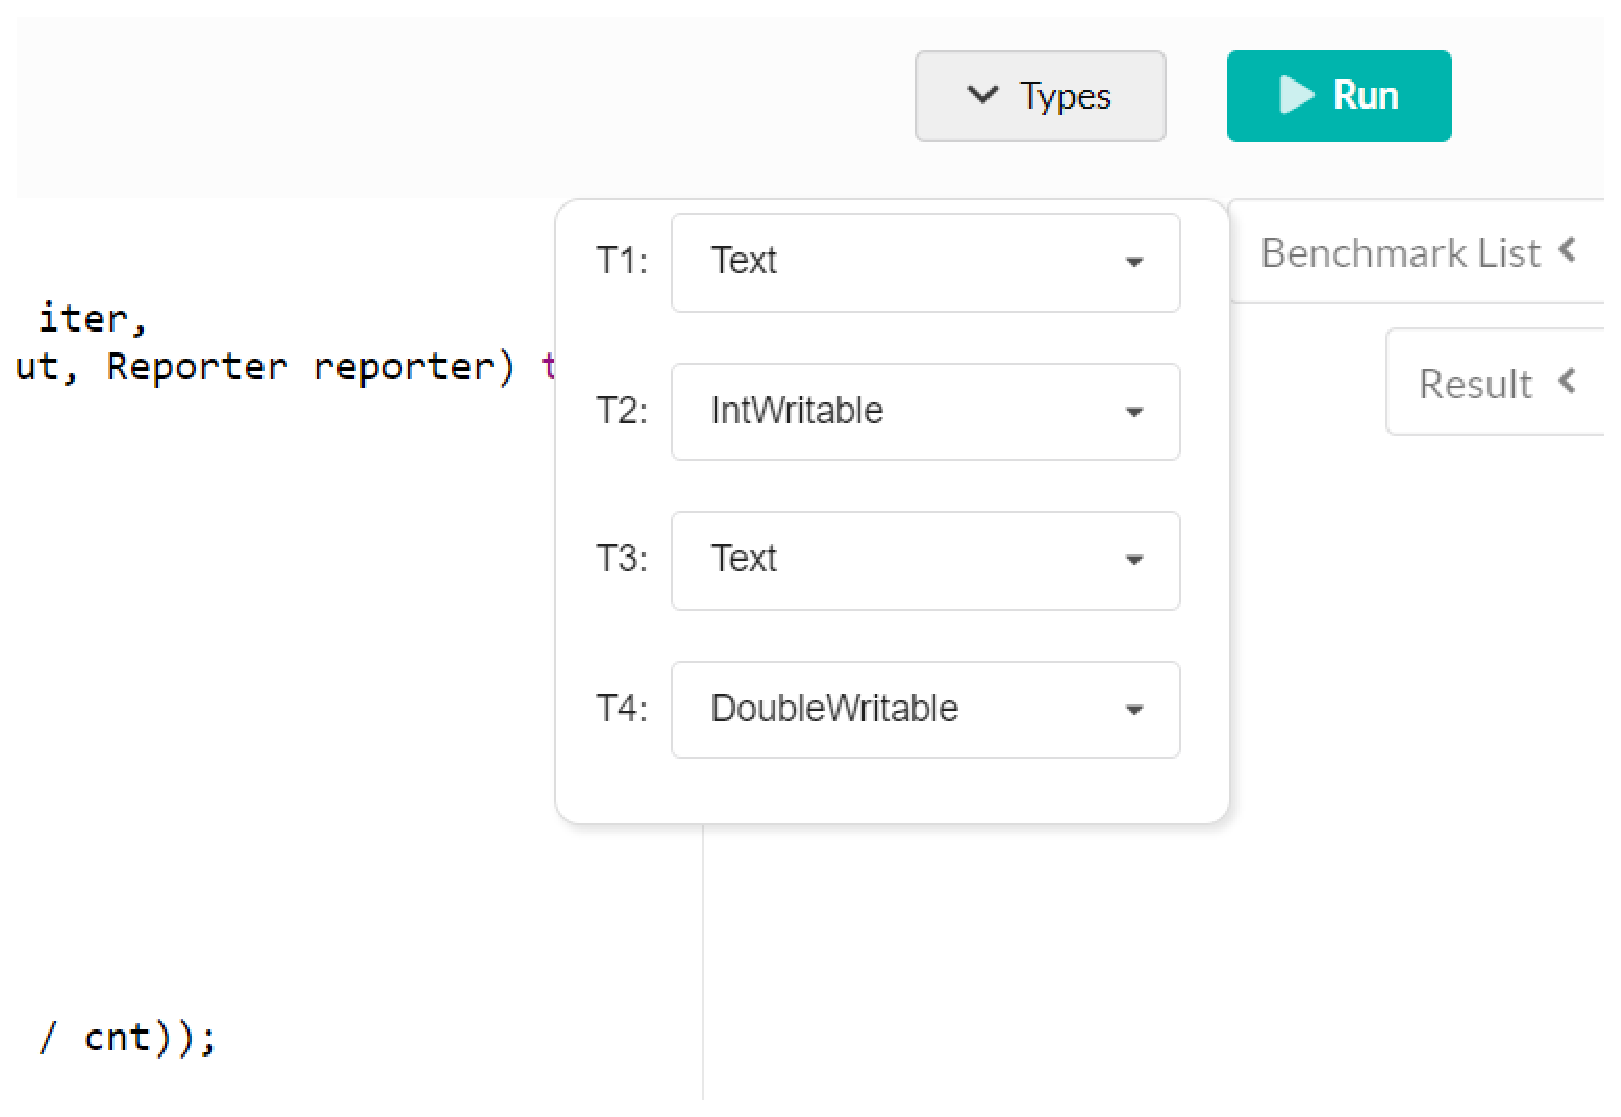
\includegraphics[width=.8\linewidth]{screenshots/type_select_menu.eps}
% \vspace{-5pt}
\caption{Type select menu}
\label{fig:type_select_menu}
% \vspace{-15pt}
\end{center}
\end{figure}

\begin{figure}
\begin{center}
% \vspace{-10pt}
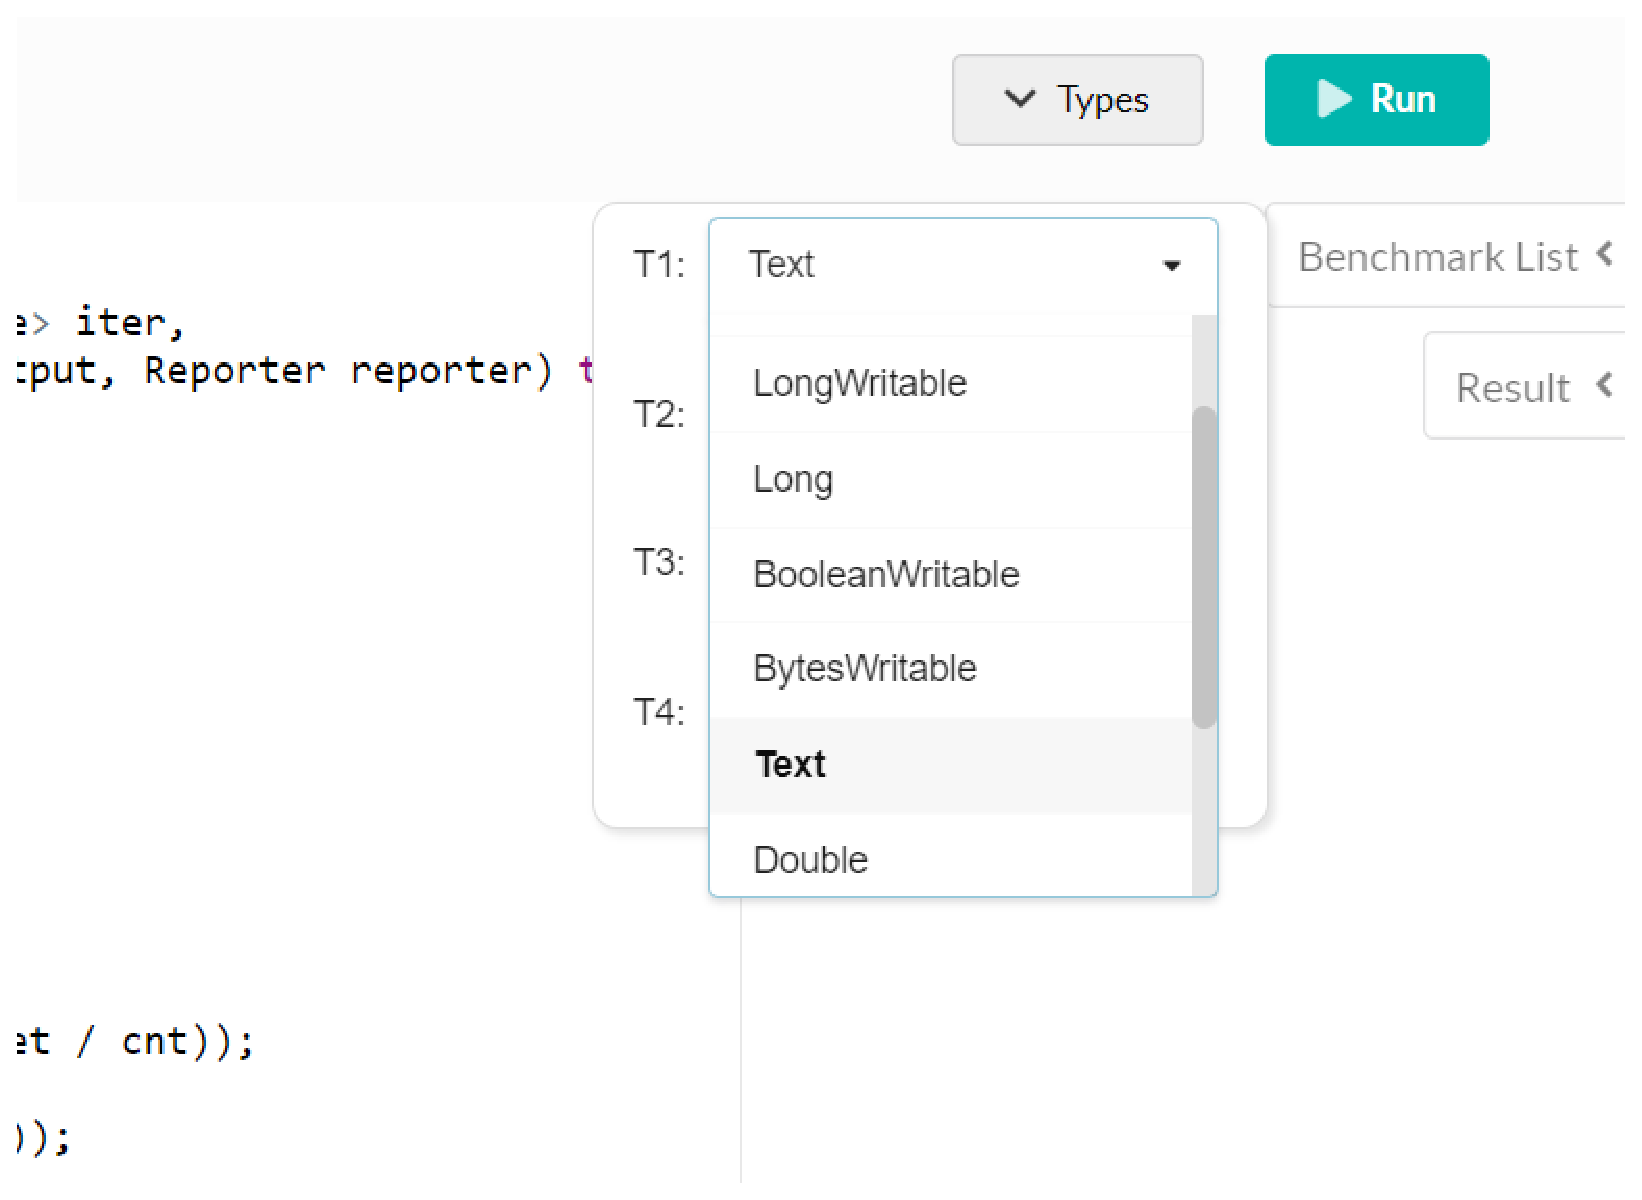
\includegraphics[width=.8\linewidth]{screenshots/selectable_types.eps}
% \vspace{-5pt}
\caption{Selectable types (part)}
\label{fig:selectable_types}
% \vspace{-15pt}
\end{center}
\end{figure}

After J-ReCoVer finishes the analysis, the \emph{"Result:"} tab of the right menu will show the result as Fig.~\ref{fig:analysis_result} shows. Fig.~\ref{fig:analysis_result_text} shows the analysis result of the first benchmark \texttt{dis.java} in detail.

\begin{figure}
\begin{center}
% \vspace{-10pt}
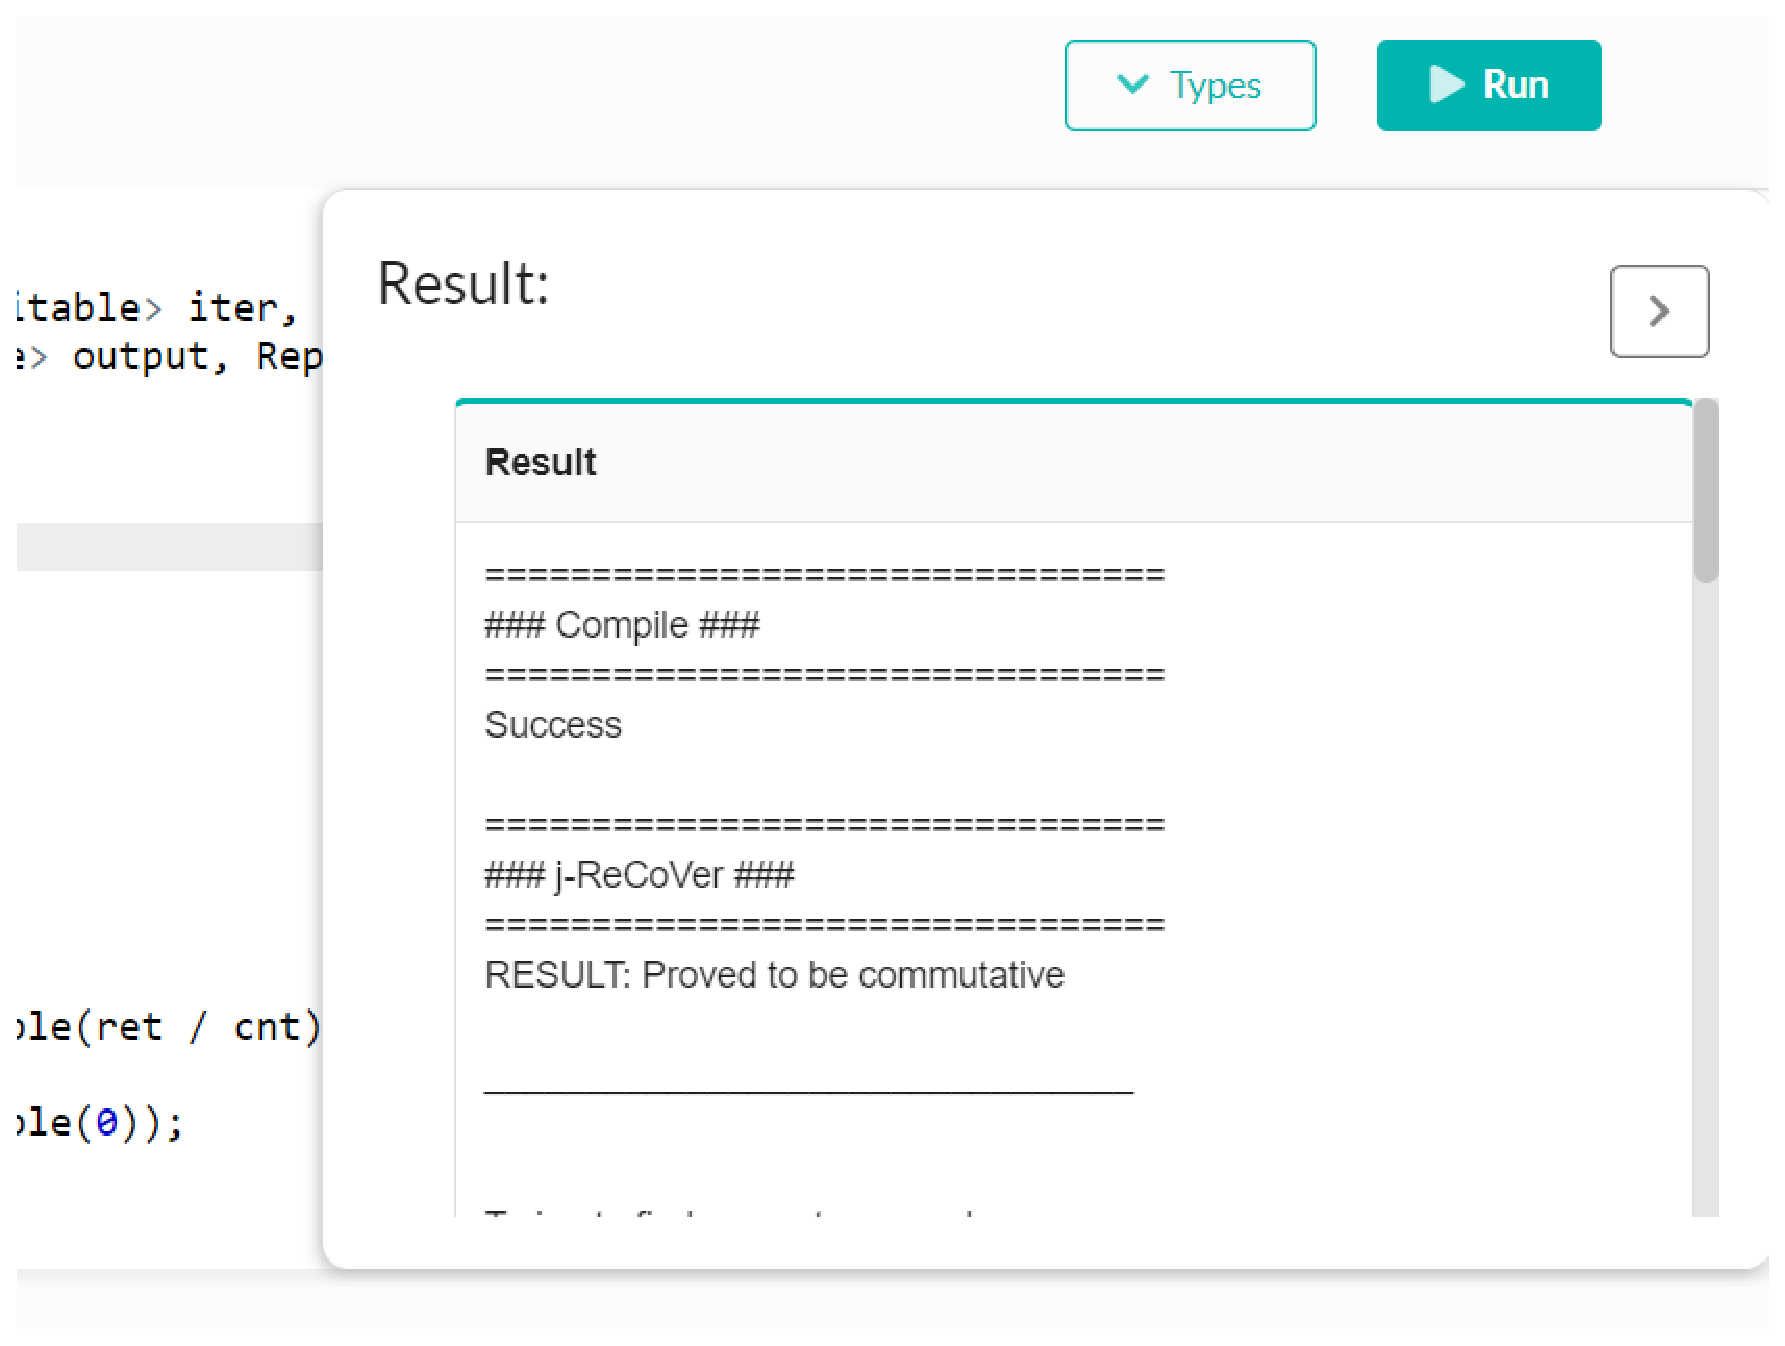
\includegraphics[width=.8\linewidth]{screenshots/analysis_result.eps}
% \vspace{-5pt}
\caption{The analysis result}
\label{fig:analysis_result}
% \vspace{-15pt}
\end{center}
\end{figure}

\begin{figure}
\begin{center}
\begin{mdframed}[roundcorner=5pt]
\begin{Verbatim}[fontsize=\tiny]
================================
### Compile ###
================================
Success

================================
### j-ReCoVer ###
================================
RESULT: Proved to be commutative

________________________________


Trying to find a counterexample...

RESULT: Cannot find a counterexample in 500 tests
Testcases were generated randomly.

Following are the first 50 lines of testcases:
Input1: o [5, 4, 5, 2, -1]
Input2: o [-1, 4, 5, 5, 2]
Output1: 

Key: [o]
Val: [0.0]
--
Output2: 

Key: [o]
Val: [0.0]
--------
Input1: j [1, -1, 0, 3, -2]
Input2: j [0, 3, -2, 1, -1]
Output1: 

Key: [j]
Val: [0.0]
--
Output2: 

Key: [j]
Val: [0.0]
--------
Input1: e [4, 3, 5, -4, 1]
Input2: e [4, -4, 5, 3, 1]
Output1: 

Key: [e]
Val: [0.0]
--
Output2: 

Key: [e]
Val: [0.0]
--------
Input1: s [3, 0, 2, -4, -1]
Input2: s [3, -1, 0, -4, 2]
Output1: 

Key: [s]
Val: [0.0]
--
Output2: 

Key: [s]
Val: [0.0]
--------
Input1: v [-3, -2, 3, 3, -3]
Input2: v [3, -2, -3, -3, 3]
\end{Verbatim}
\end{mdframed}
\caption{The analysis result of \texttt{dis.java}}
\label{fig:analysis_result_text}
\end{center}
\end{figure}

In a commutativity analysis, J-ReCoVer first tries to compile the example then perfrom commutativity analysis. If the analysis says the example is commutative, J-ReCoVer then runs 500 randomly generated test cases to try to find a counterexample. If the test cases all pass, J-ReCoVer concludes that the example is commutative, or the result will be "unknown" since the results of analysis and tests are inconsistent. For the case that the commutativity analysis returns false, J-ReCoVer will also run test cases to find a counterexample. This time, J-ReCoVer will conclude "not commutative" if a counterexample is found, or "unknown" if no counterexample is found. 

\subsection{Run Analysis of an example from sketch}
\label{appendix:3}

Besides examples from the benchmark, J-ReCoVer also provides an interactive way to analyze a reduce function starting from a sketch.
The upper-left menu (below the top menu) provides blank templates for two versions of Hadoop. The templates are

\begin{mdframed}[roundcorner=5pt]
\begin{verbatim}
public void reduce(T1 key, Iterator<T2> values,
	OutputCollector<T3,T4> oc1, Reporter reporter)
		throws IOException,InterruptedException {

}
\end{verbatim}
\end{mdframed}

, and

\begin{mdframed}[roundcorner=5pt]
\begin{verbatim}
public void reduce(T1 key, Iterable<T2> values,
	Context context) throws IOException,InterruptedException {

}
\end{verbatim}
\end{mdframed}

In this case, one would have to manually fill the types T1 to T4 and the function body, then selects the types from the pull-down menu, as shown in Fig.~\ref{fig:type_select_menu} and Fig.~\ref{fig:selectable_types}.

For more details, all selectable types are:

\begin{itemize}
\item Long
\item BooleanWritable
\item BytesWritable
\item Text
\item Double
\item DoubleWritable
\item Float
\item FloatWritable
\end{itemize}

\clearpage
\appendix

\section{J-ReCoVer Usages}

\subsection{The User Interface of J-ReCoVer}
\label{appendix:1}

J-ReCoVer is available online at \url{\texttt{http://jrecover.iis.sinica.edu.tw/}}. Fig.~\ref{fig:main_screen} shows the main screen of J-ReCoVer. The alignment of user interface elements are as follows:

\begin{figure}
\begin{center}
% \vspace{-10pt}
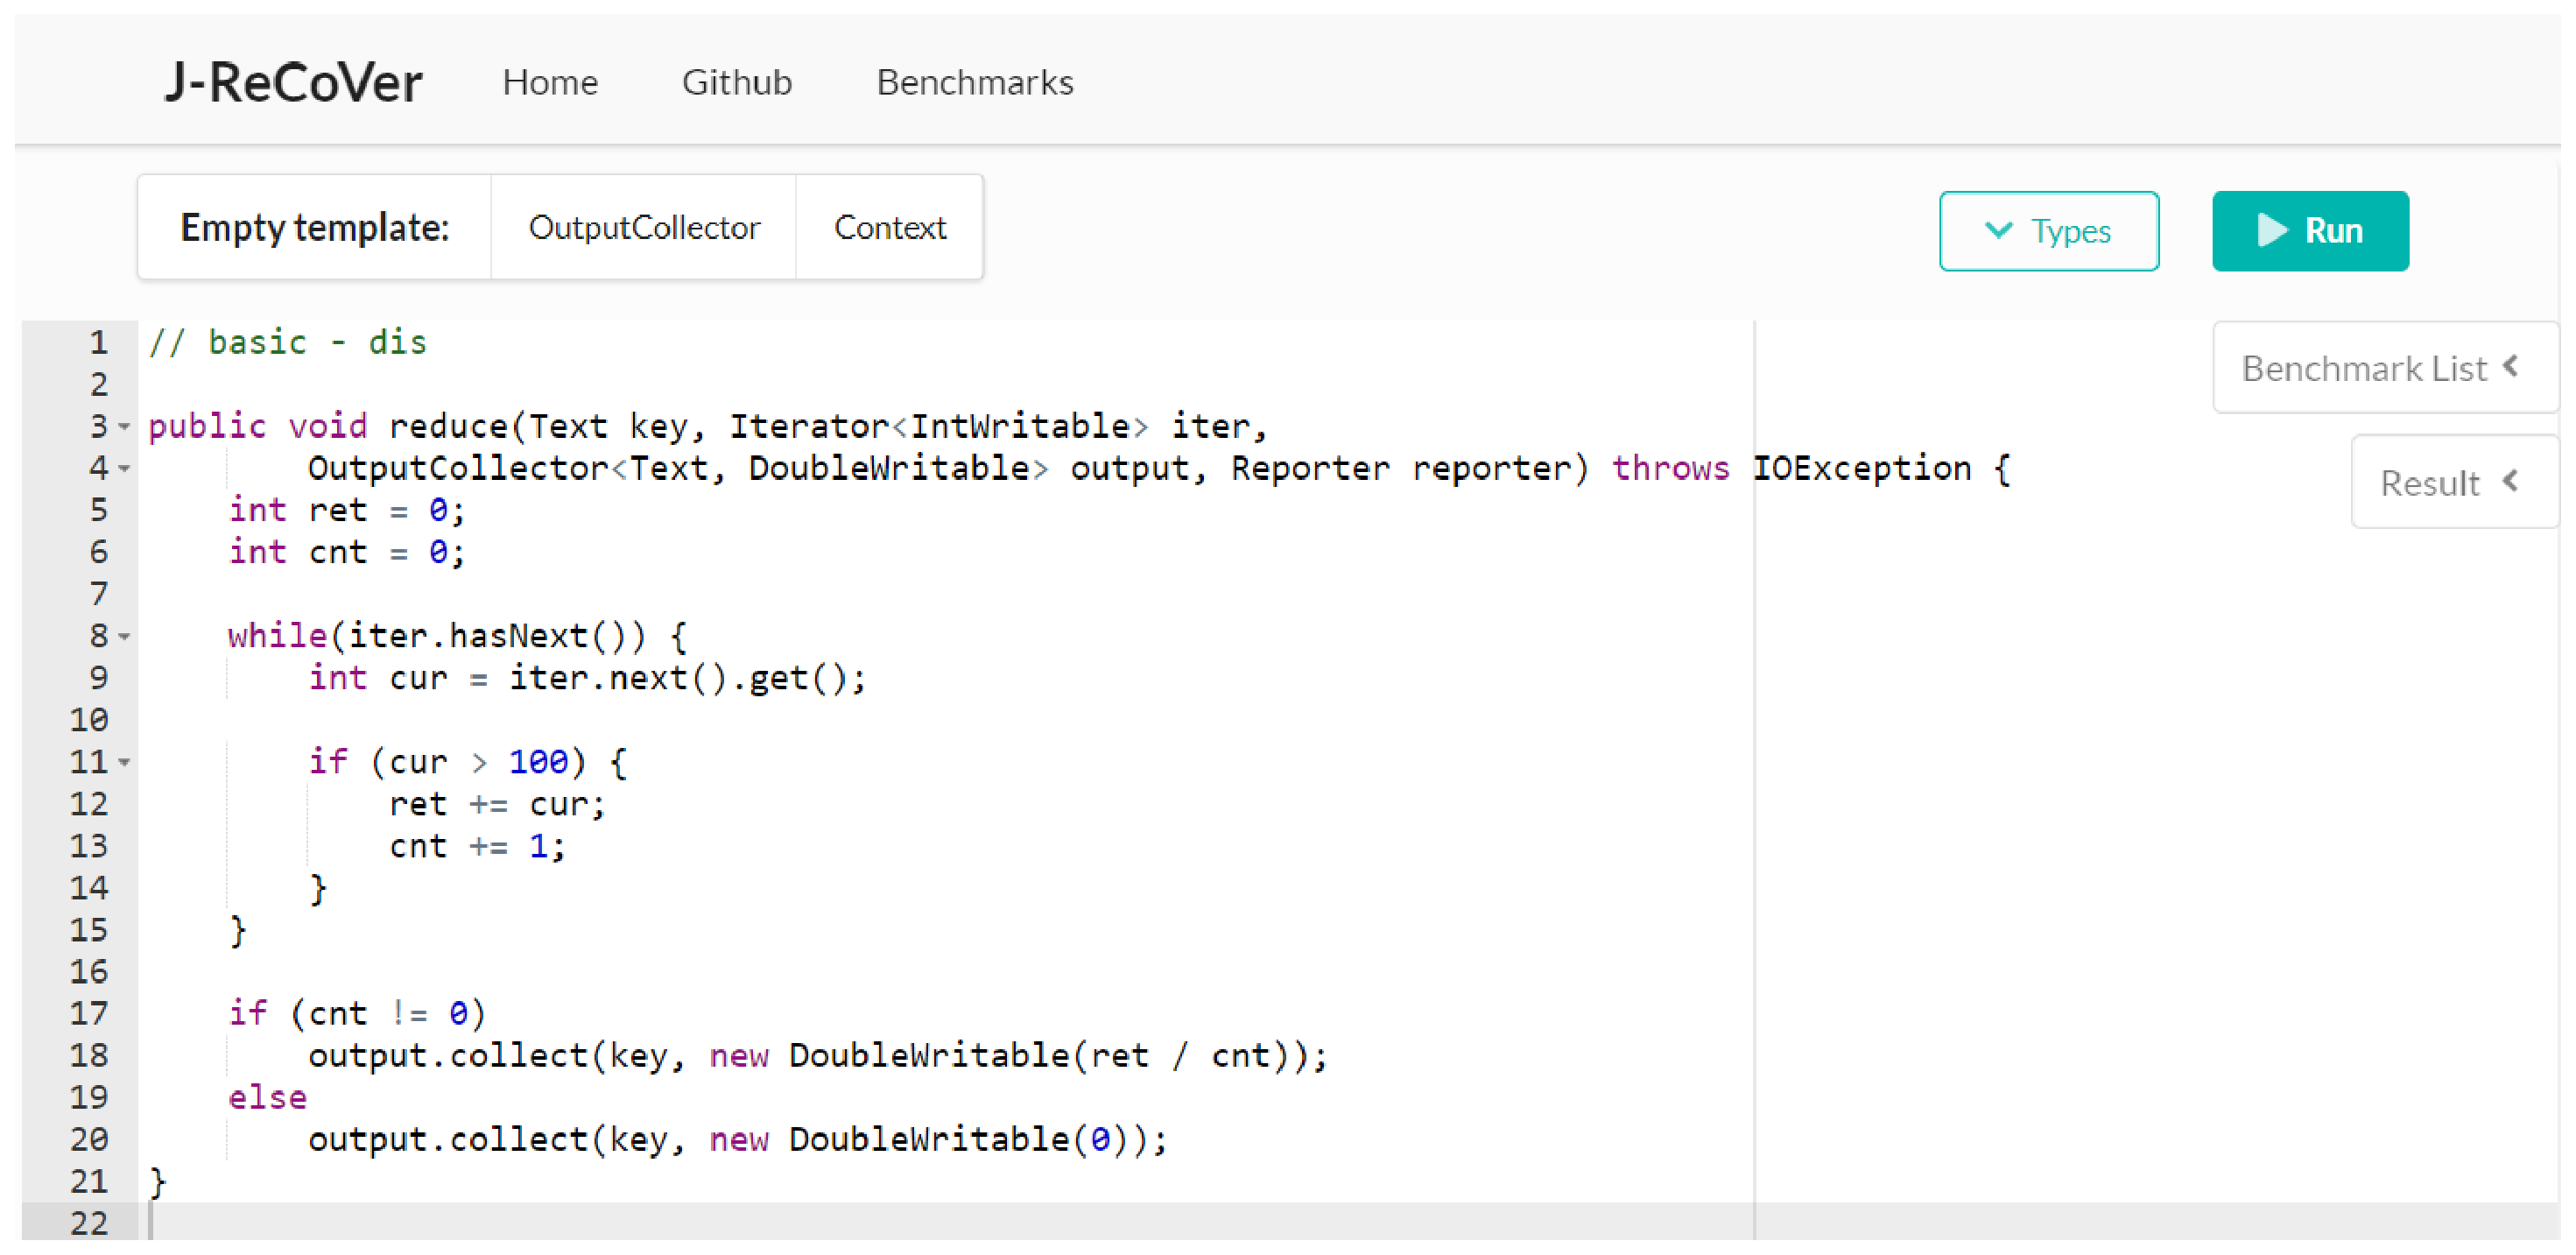
\includegraphics[width=.9\linewidth]{screenshots/main_screen.eps}
% \vspace{-5pt}
\caption{Main Screen of J-ReCoVer}
\label{fig:main_screen}
% \vspace{-15pt}
\end{center}
\end{figure}

\begin{itemize}
\item
Top Menu:
\begin{itemize}
\item
\emph{"Github"} opens a new tab of the repository of J-ReCoVer. The repository also has source code of benchmarks.
\item
\emph{"Benchmark"} leads to the list of benchmarks we collected with their results of commutativity analysis as Fig.~\ref{fig:benchmark_list} shows. Select the filename or "try it" button will select the example and go back to the main screen.
\end{itemize}
\item
Right Menu:
\begin{itemize}
\item
\emph{"Benchmark List"} provides a quick selection to examples in the benchmark (Fig.~\ref{fig:benchmark_list_right})
\item
\emph{"Results"} shows the last analysis result.
\end{itemize}
\item
Upper-Right Menu:
\begin{itemize}
\item
\emph{"Type"} provides types that J-ReCoVer supports. Details are explained in~\ref{appendix:3}.
\item
\emph{"Run"} starts the analysis of the selected example.
\end{itemize}
\item
Upper-Left Menu: See~\ref{appendix:3}.
\end{itemize}

\begin{figure}
\begin{center}
% \vspace{-10pt}
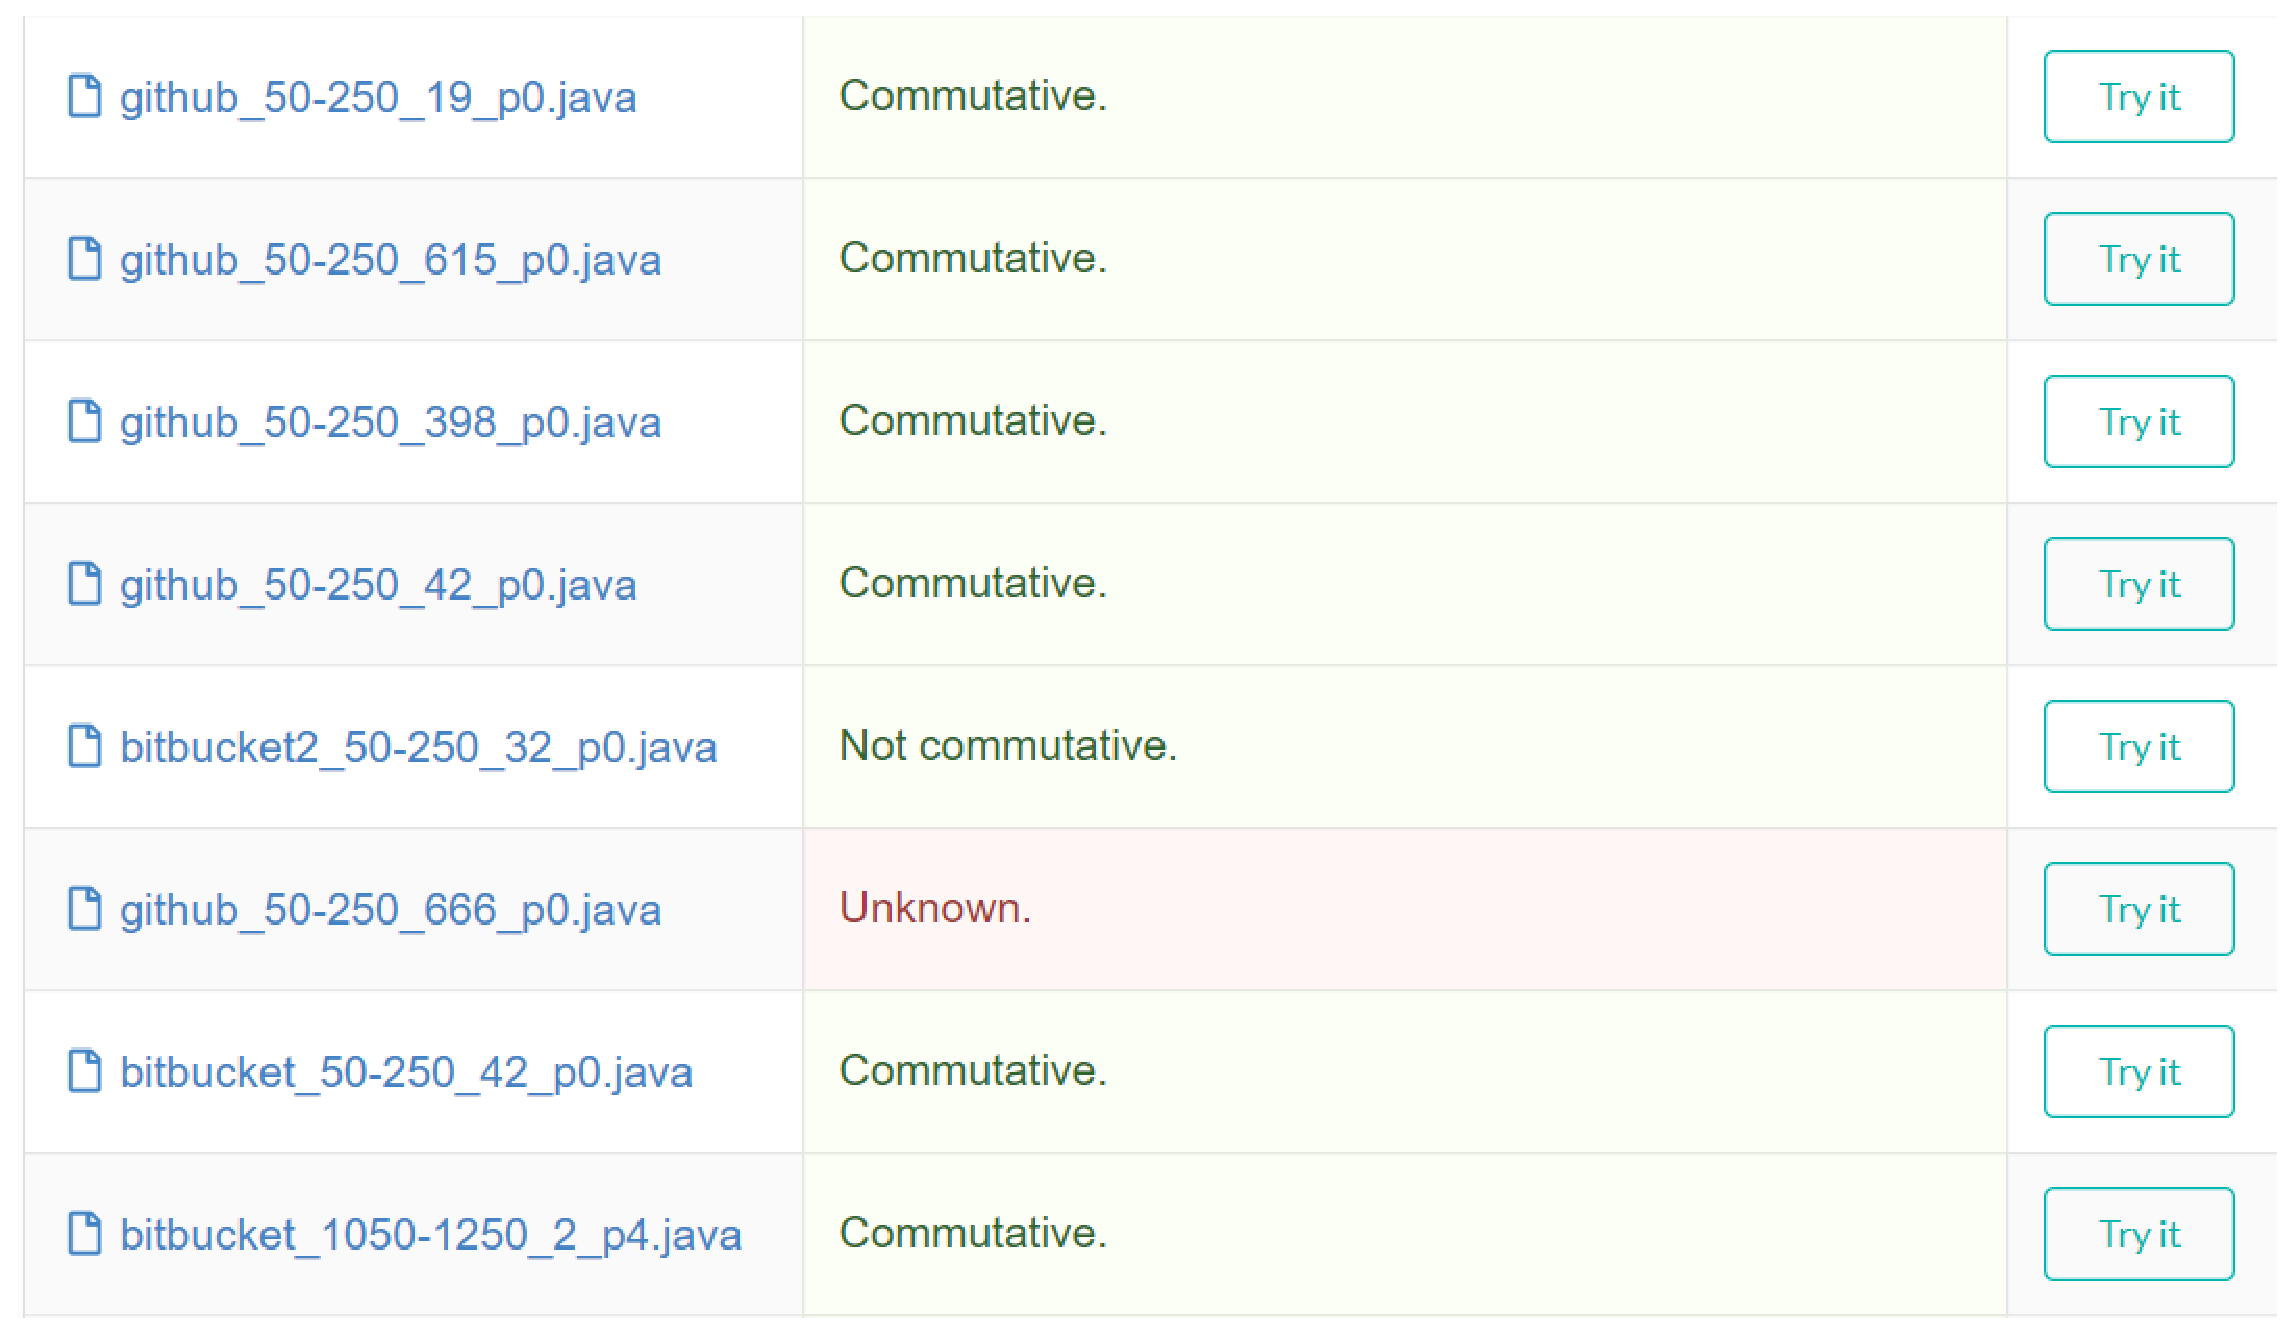
\includegraphics[width=.8\linewidth]{screenshots/benchmark_list.eps}
% \vspace{-5pt}
\caption{Benchmark list from top menu (part)}
\label{fig:benchmark_list}
% \vspace{-15pt}
\end{center}
\end{figure}

\begin{figure}
\begin{center}
% \vspace{-10pt}
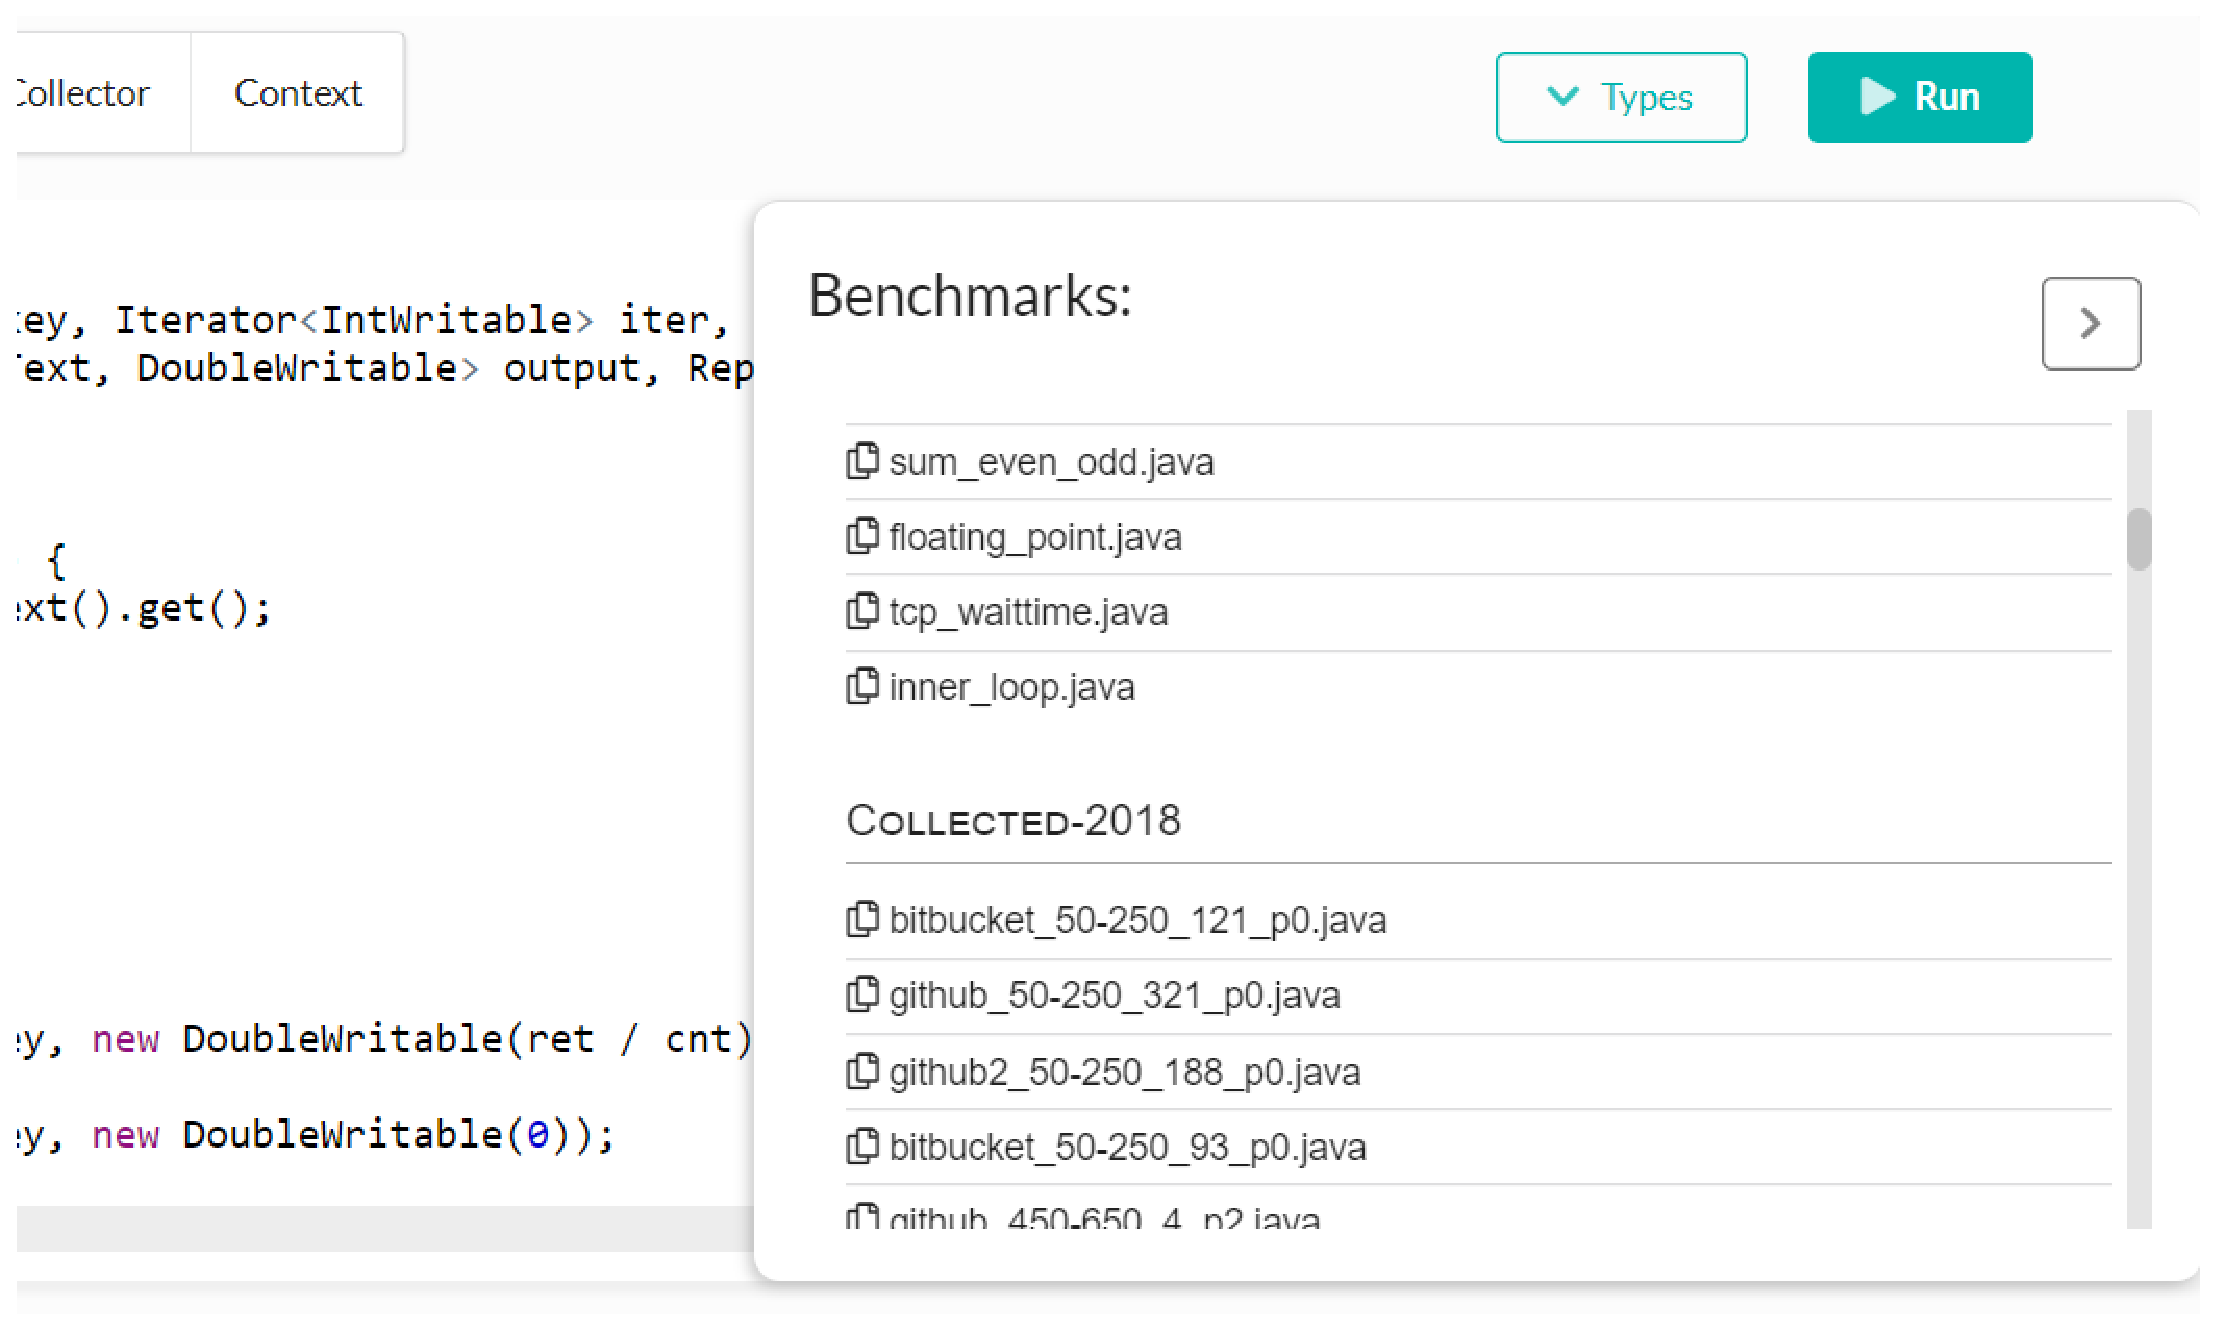
\includegraphics[width=.8\linewidth]{screenshots/benchmark_list_right.eps}
% \vspace{-5pt}
\caption{Benchmark list from right menu (part)}
\label{fig:benchmark_list_right}
% \vspace{-15pt}
\end{center}
\end{figure}

\subsection{Run analysis of selected benchmark example}
\label{appendix:2}

To run analysis, you can choose an example from benchmark using either the top menu or the right menu, then click the "Run" button of the upper-right menu to start the commutativity analysis of the selected example. The pull-down menu "Types" of the upper-right menu provides selectable types for input \texttt{(T1,T2)} and output \texttt{(T3,T4)}. Fig.~\ref{fig:type_select_menu} shows the pull-down menu and Fig.~\ref{fig:selectable_types} shows part of the selectable types in J-ReCoVer. If one selects an example from the benchmark, the types will be automatically selected to match the example. The selection will be needed if the user wants to write a reduce function from sketch for analysis (see~\ref{appendix:3}).

\begin{figure}
\begin{center}
% \vspace{-10pt}
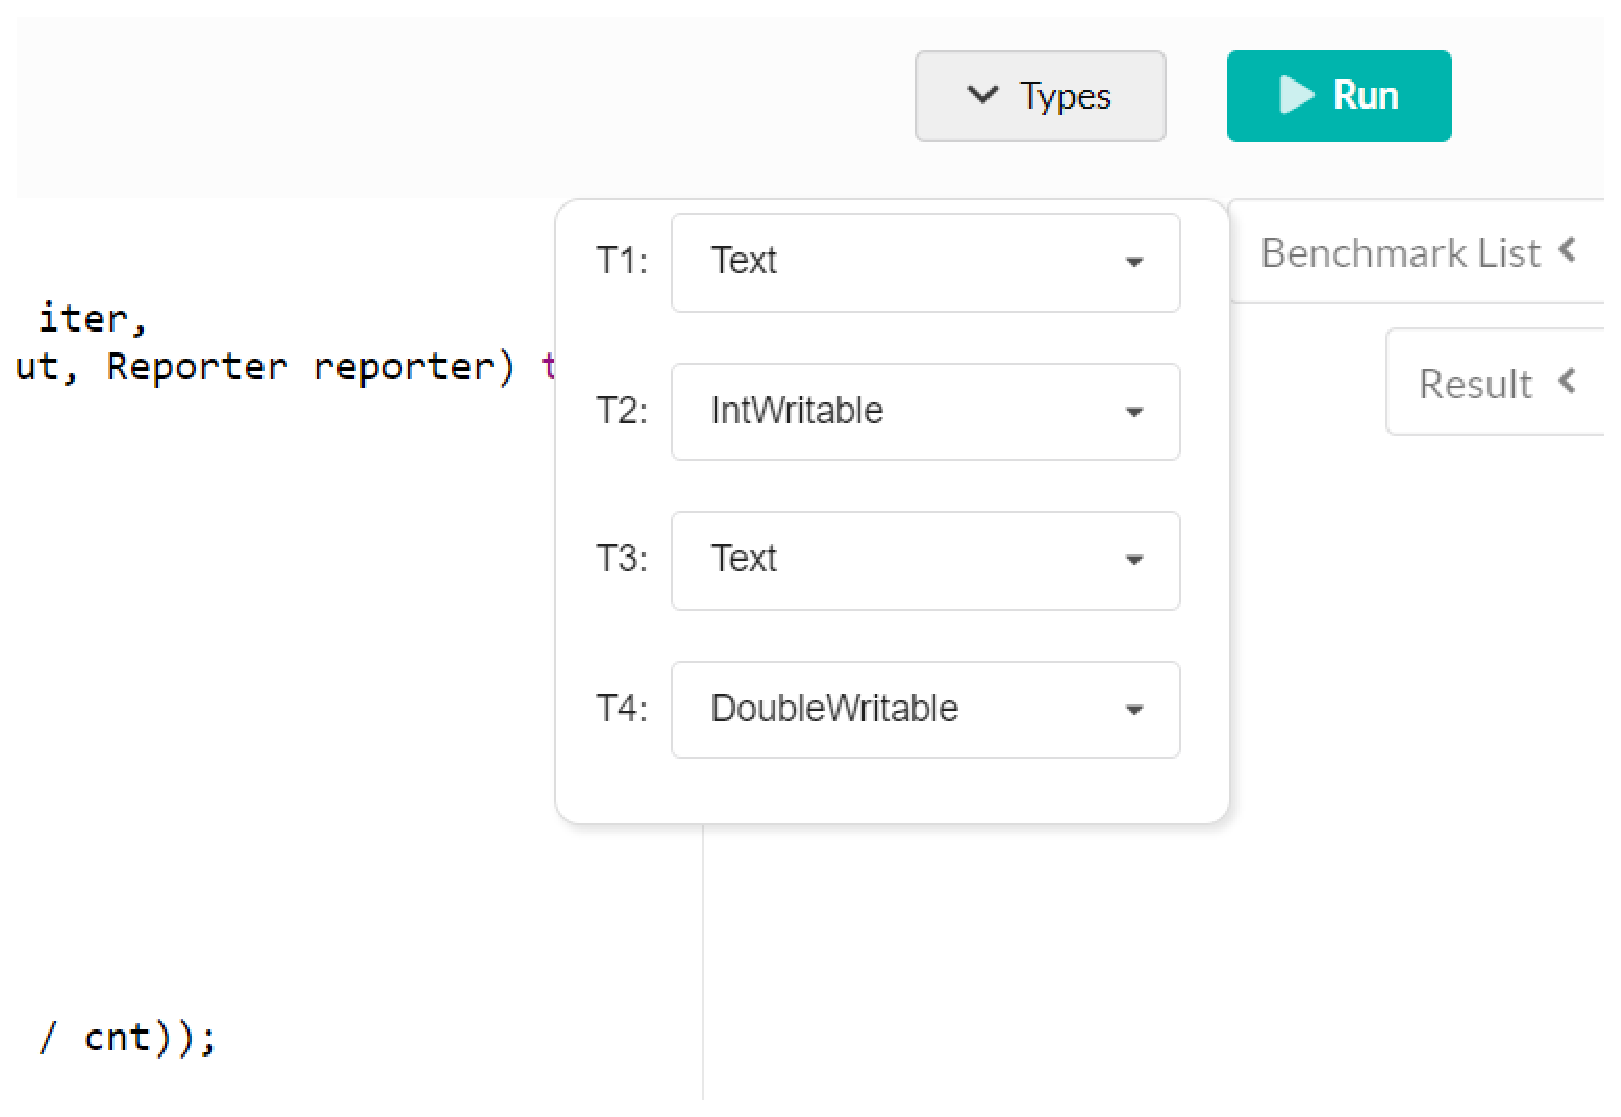
\includegraphics[width=.8\linewidth]{screenshots/type_select_menu.eps}
% \vspace{-5pt}
\caption{Type select menu}
\label{fig:type_select_menu}
% \vspace{-15pt}
\end{center}
\end{figure}

\begin{figure}
\begin{center}
% \vspace{-10pt}
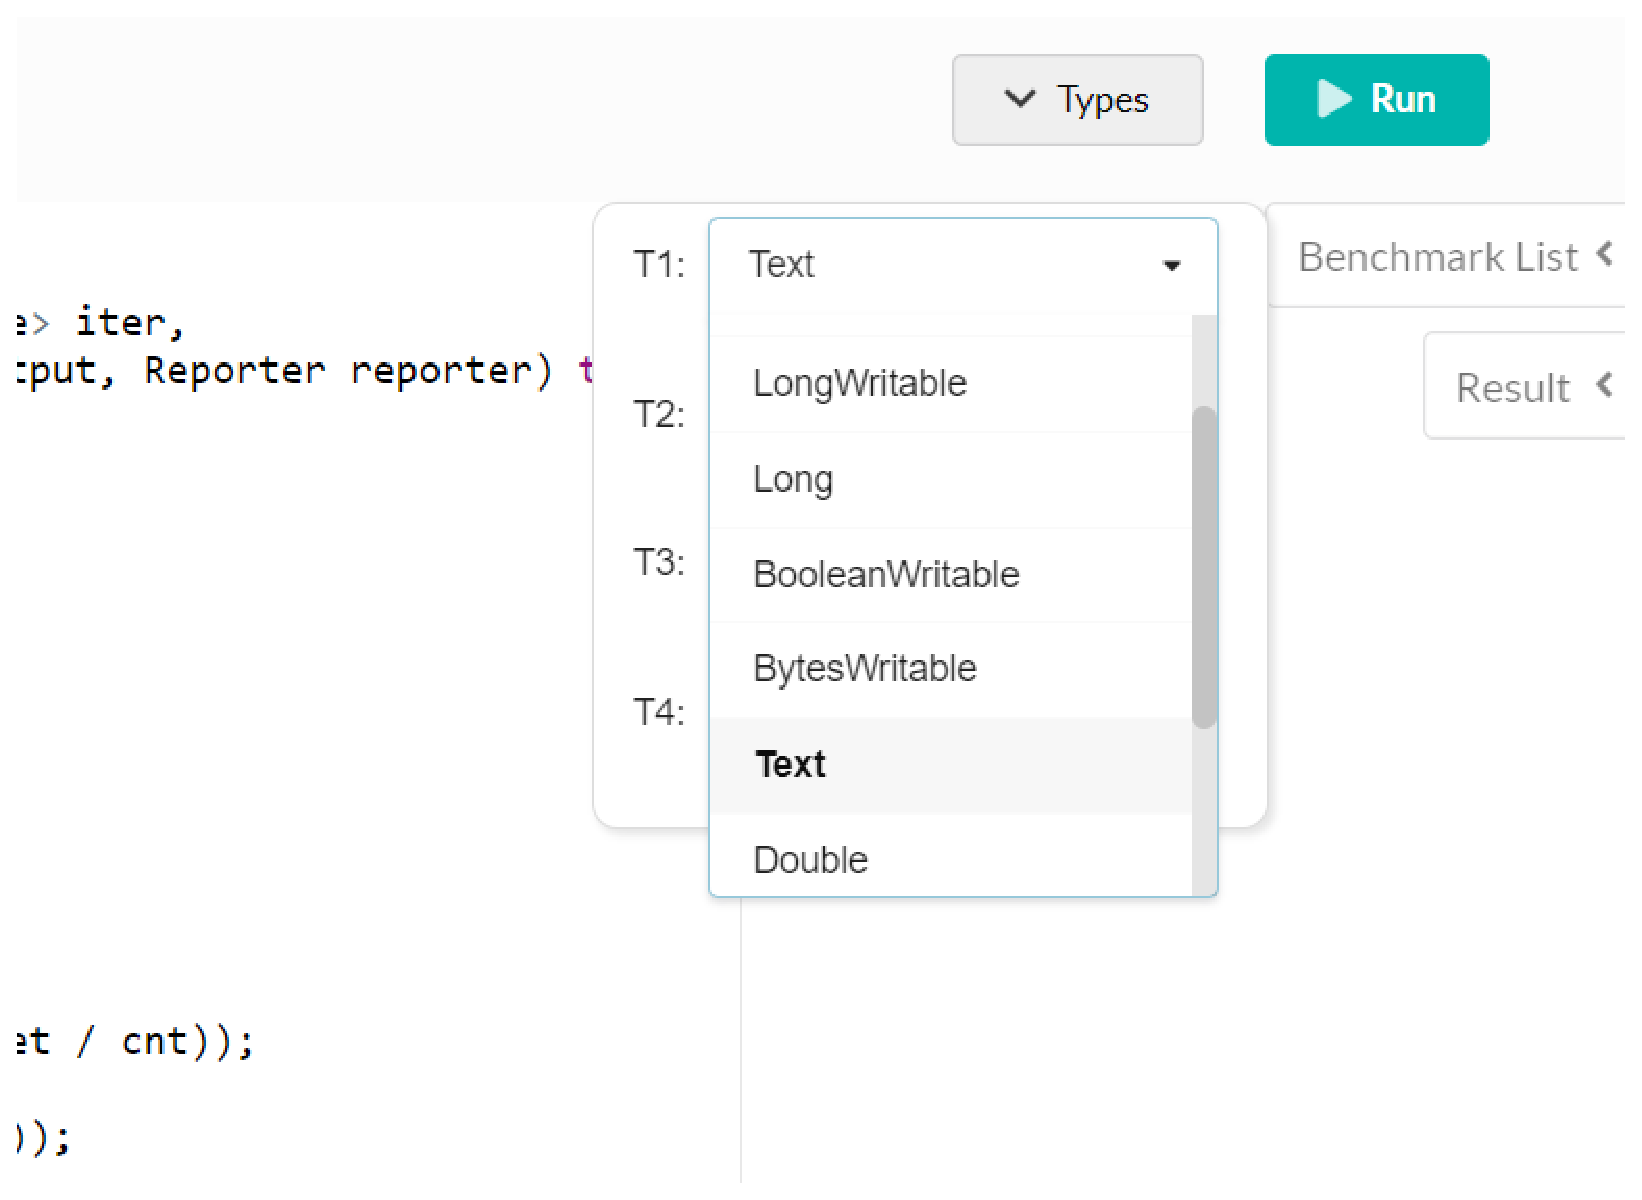
\includegraphics[width=.8\linewidth]{screenshots/selectable_types.eps}
% \vspace{-5pt}
\caption{Selectable types (part)}
\label{fig:selectable_types}
% \vspace{-15pt}
\end{center}
\end{figure}

After J-ReCoVer finishes the analysis, the \emph{"Result:"} tab of the right menu will show the result as Fig.~\ref{fig:analysis_result} shows. Fig.~\ref{fig:analysis_result_text} shows the analysis result of the first benchmark \texttt{dis.java} in detail.

\begin{figure}
\begin{center}
% \vspace{-10pt}
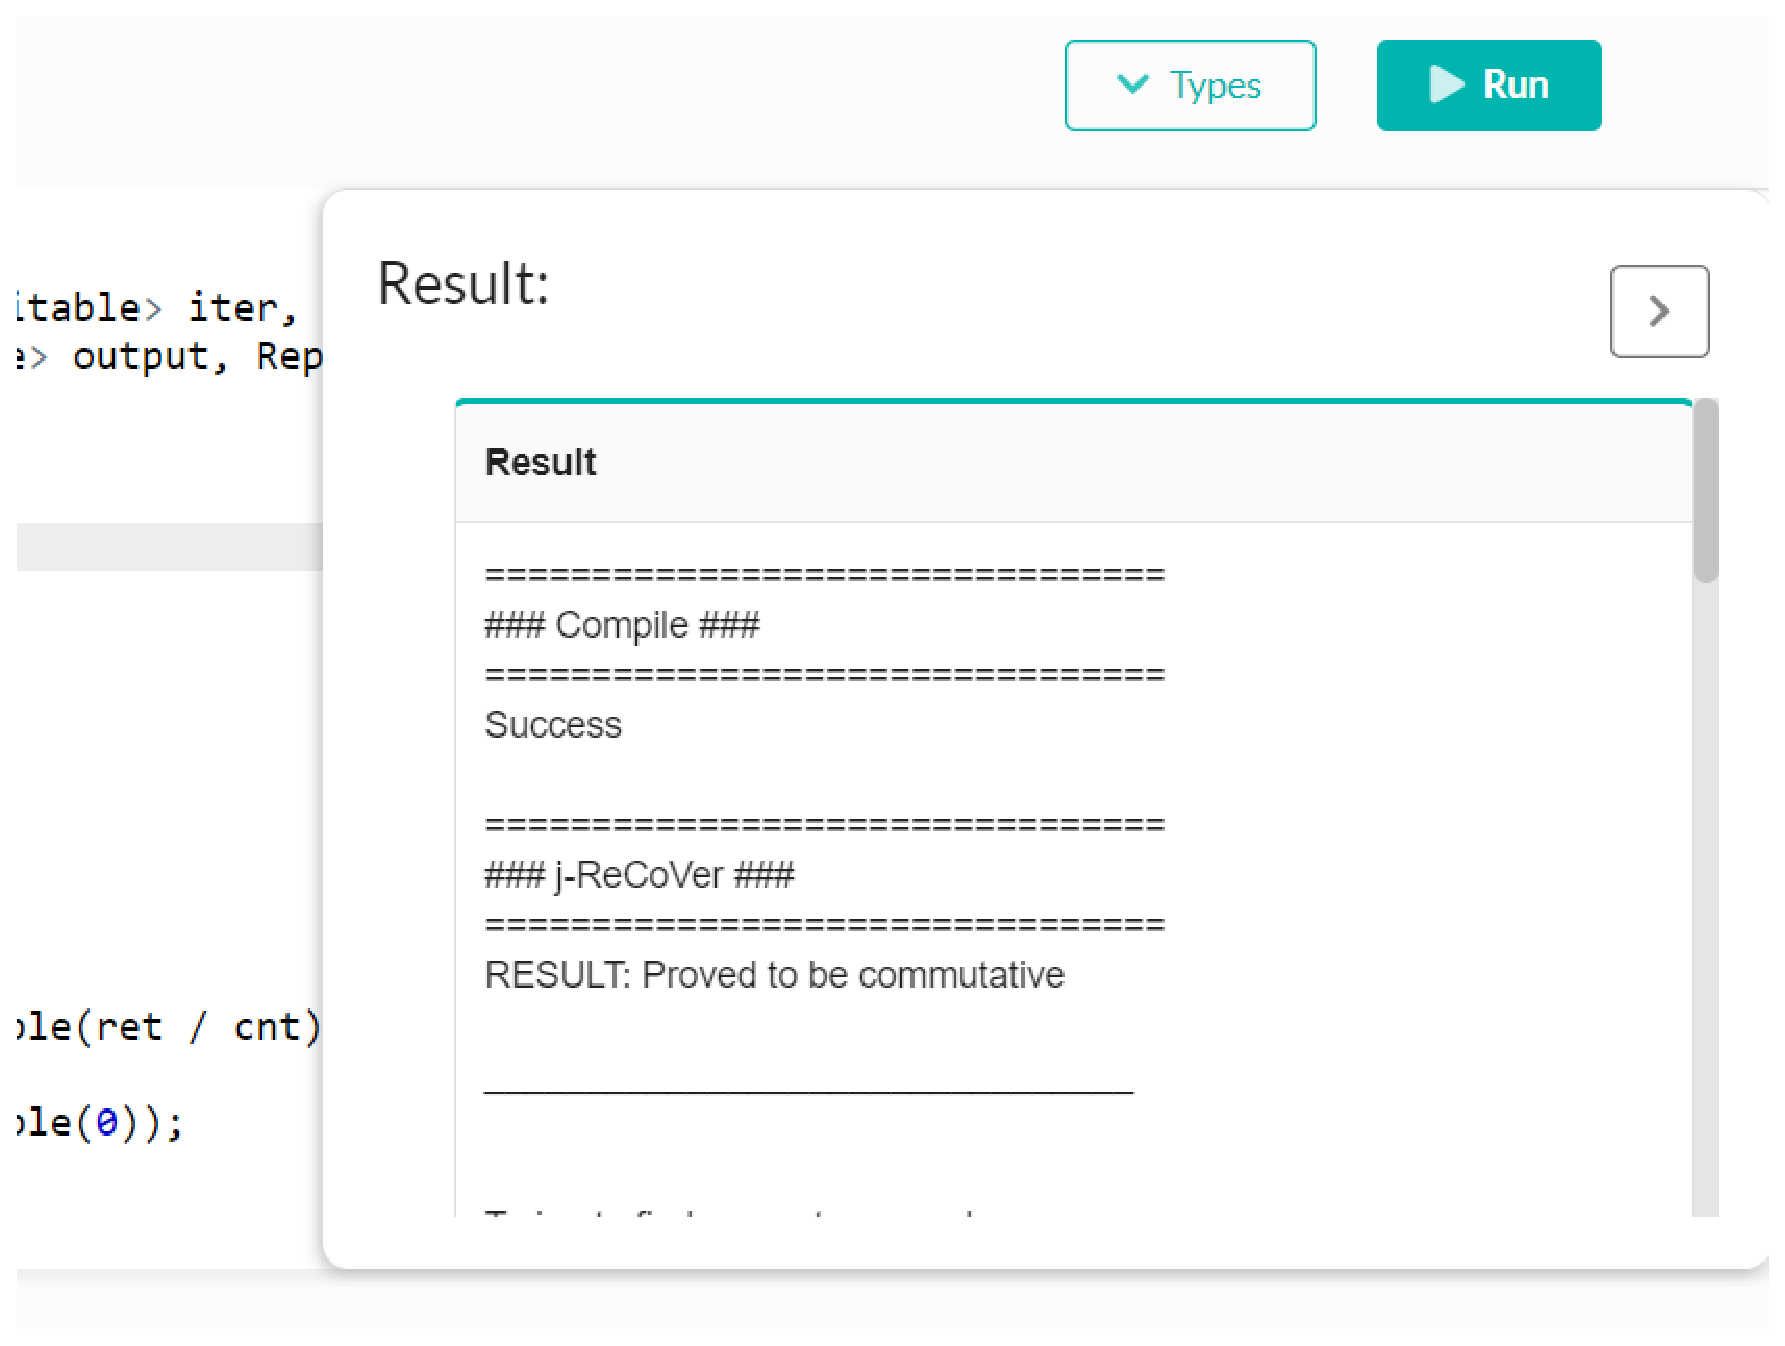
\includegraphics[width=.8\linewidth]{screenshots/analysis_result.eps}
% \vspace{-5pt}
\caption{The analysis result}
\label{fig:analysis_result}
% \vspace{-15pt}
\end{center}
\end{figure}

\begin{figure}
\begin{center}
\begin{mdframed}[roundcorner=5pt]
\begin{Verbatim}[fontsize=\tiny]
================================
### Compile ###
================================
Success

================================
### j-ReCoVer ###
================================
RESULT: Proved to be commutative

________________________________


Trying to find a counterexample...

RESULT: Cannot find a counterexample in 500 tests
Testcases were generated randomly.

Following are the first 50 lines of testcases:
Input1: o [5, 4, 5, 2, -1]
Input2: o [-1, 4, 5, 5, 2]
Output1: 

Key: [o]
Val: [0.0]
--
Output2: 

Key: [o]
Val: [0.0]
--------
Input1: j [1, -1, 0, 3, -2]
Input2: j [0, 3, -2, 1, -1]
Output1: 

Key: [j]
Val: [0.0]
--
Output2: 

Key: [j]
Val: [0.0]
--------
Input1: e [4, 3, 5, -4, 1]
Input2: e [4, -4, 5, 3, 1]
Output1: 

Key: [e]
Val: [0.0]
--
Output2: 

Key: [e]
Val: [0.0]
--------
Input1: s [3, 0, 2, -4, -1]
Input2: s [3, -1, 0, -4, 2]
Output1: 

Key: [s]
Val: [0.0]
--
Output2: 

Key: [s]
Val: [0.0]
--------
Input1: v [-3, -2, 3, 3, -3]
Input2: v [3, -2, -3, -3, 3]
\end{Verbatim}
\end{mdframed}
\caption{The analysis result of \texttt{dis.java}}
\label{fig:analysis_result_text}
\end{center}
\end{figure}

In a commutativity analysis, J-ReCoVer first tries to compile the example then perfrom commutativity analysis. If the analysis says the example is commutative, J-ReCoVer then runs 500 randomly generated test cases to try to find a counterexample. If the test cases all pass, J-ReCoVer concludes that the example is commutative, or the result will be "unknown" since the results of analysis and tests are inconsistent. For the case that the commutativity analysis returns false, J-ReCoVer will also run test cases to find a counterexample. This time, J-ReCoVer will conclude "not commutative" if a counterexample is found, or "unknown" if no counterexample is found. 

\subsection{Run Analysis of an example from sketch}
\label{appendix:3}

Besides examples from the benchmark, J-ReCoVer also provides an interactive way to analyze a reduce function starting from a sketch.
The upper-left menu (below the top menu) provides blank templates for two versions of Hadoop. The templates are

\begin{mdframed}[roundcorner=5pt]
\begin{verbatim}
public void reduce(T1 key, Iterator<T2> values,
	OutputCollector<T3,T4> oc1, Reporter reporter)
		throws IOException,InterruptedException {

}
\end{verbatim}
\end{mdframed}

, and

\begin{mdframed}[roundcorner=5pt]
\begin{verbatim}
public void reduce(T1 key, Iterable<T2> values,
	Context context) throws IOException,InterruptedException {

}
\end{verbatim}
\end{mdframed}

In this case, one would have to manually fill the types T1 to T4 and the function body, then selects the types from the pull-down menu, as shown in Fig.~\ref{fig:type_select_menu} and Fig.~\ref{fig:selectable_types}.

For more details, all selectable types are:

\begin{itemize}
\item Long
\item BooleanWritable
\item BytesWritable
\item Text
\item Double
\item DoubleWritable
\item Float
\item FloatWritable
\end{itemize}

\clearpage
\appendix

\section{J-ReCoVer Demo}

Our plan is to demonstrate the basic usage of J-ReCoVer on two examples. The
first example is a reducer that is not commutative, and J-ReCoVer will report a
counterexample. Based on this counterexample, we will fix the reducer to get the
second example, and let J-ReCoVer to check it again. Now, J-ReCoVer will report
that the reducer is commutative. Below, we give a more detailed description of
the functionalities of J-ReCoVer. 

\subsection{The User Interface of J-ReCoVer}
\label{appendix:1}

Figure~\ref{fig:main_screen} shows the main screen of J-ReCoVer. 

\begin{figure}
\begin{center}
% \vspace{-10pt}
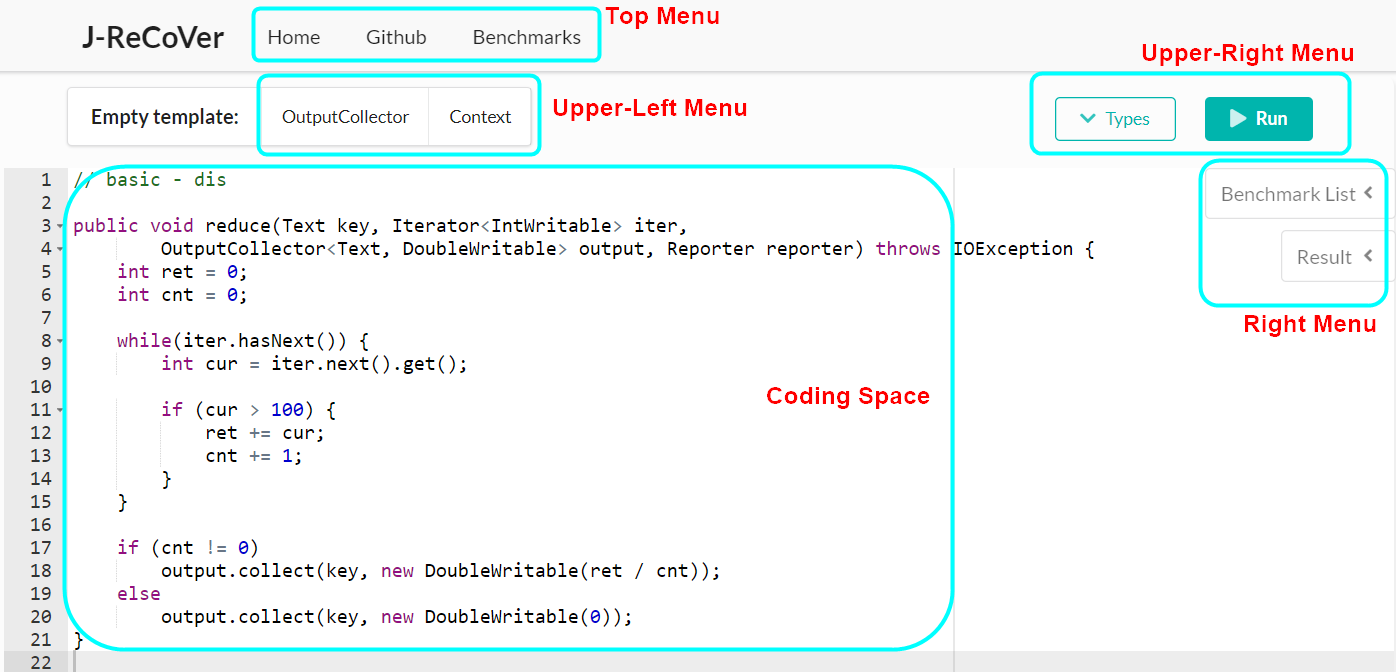
\includegraphics[width=.9\linewidth]{screenshots/main_screen_marked}
% \vspace{-5pt}
\caption{The main screen of J-ReCoVer.}
\label{fig:main_screen}
% \vspace{-15pt}
\end{center}
\end{figure}

The alignment of the user interface elements in the main screen is as follows:
\begin{itemize}
\item
Top Menu:
\begin{itemize}
\item
\emph{``GitHub''} opens a new tab of the repository of J-ReCoVer. The repository
does also contain the source code of our benchmarks.
\item
\emph{``Benchmark''} leads to the list of benchmarks we collected with their
results of commutativity analysis as Fig.~\ref{fig:benchmark_list} shows. Select
a file name or use the ``try it'' button to select an example and go back to the main screen.
\end{itemize}
\item
Right Menu:
\begin{itemize}
\item
\emph{``Benchmark List''} provides a quick selection of examples in the
benchmark (Fig.~\ref{fig:benchmark_list_right}).
\item
\emph{``Results''} shows the last analysis result.
\end{itemize}
\item
Upper-Right Menu:
\begin{itemize}
\item
\emph{``Type''} provides types that J-ReCoVer supports. Details are explained in
Appendix~\ref{appendix:3}.
\item
\emph{``Run''} starts the analysis of the selected example.
\end{itemize}
\item
Upper-Left Menu: See Appendix~\ref{appendix:3}.
\item
Coding Space.
\end{itemize}

\begin{figure}
\begin{center}
% \vspace{-10pt}
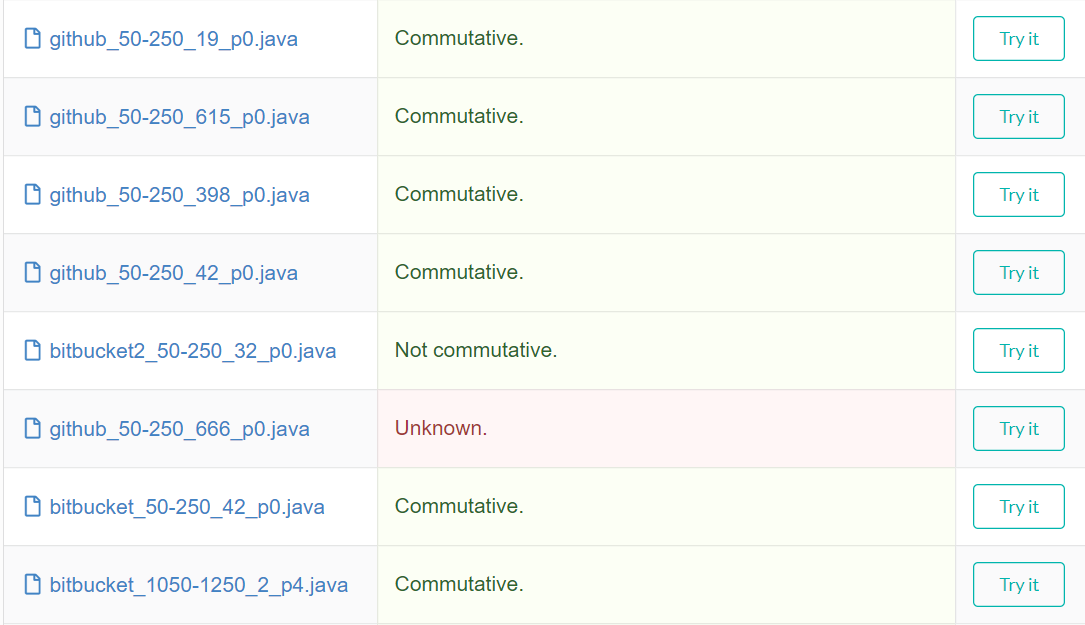
\includegraphics[width=.8\linewidth]{screenshots/benchmark_list}
% \vspace{-5pt}
\caption{A benchmark list from the top menu (a part).}
\label{fig:benchmark_list}
% \vspace{-15pt}
\end{center}
\end{figure}

\begin{figure}
\begin{center}
% \vspace{-10pt}
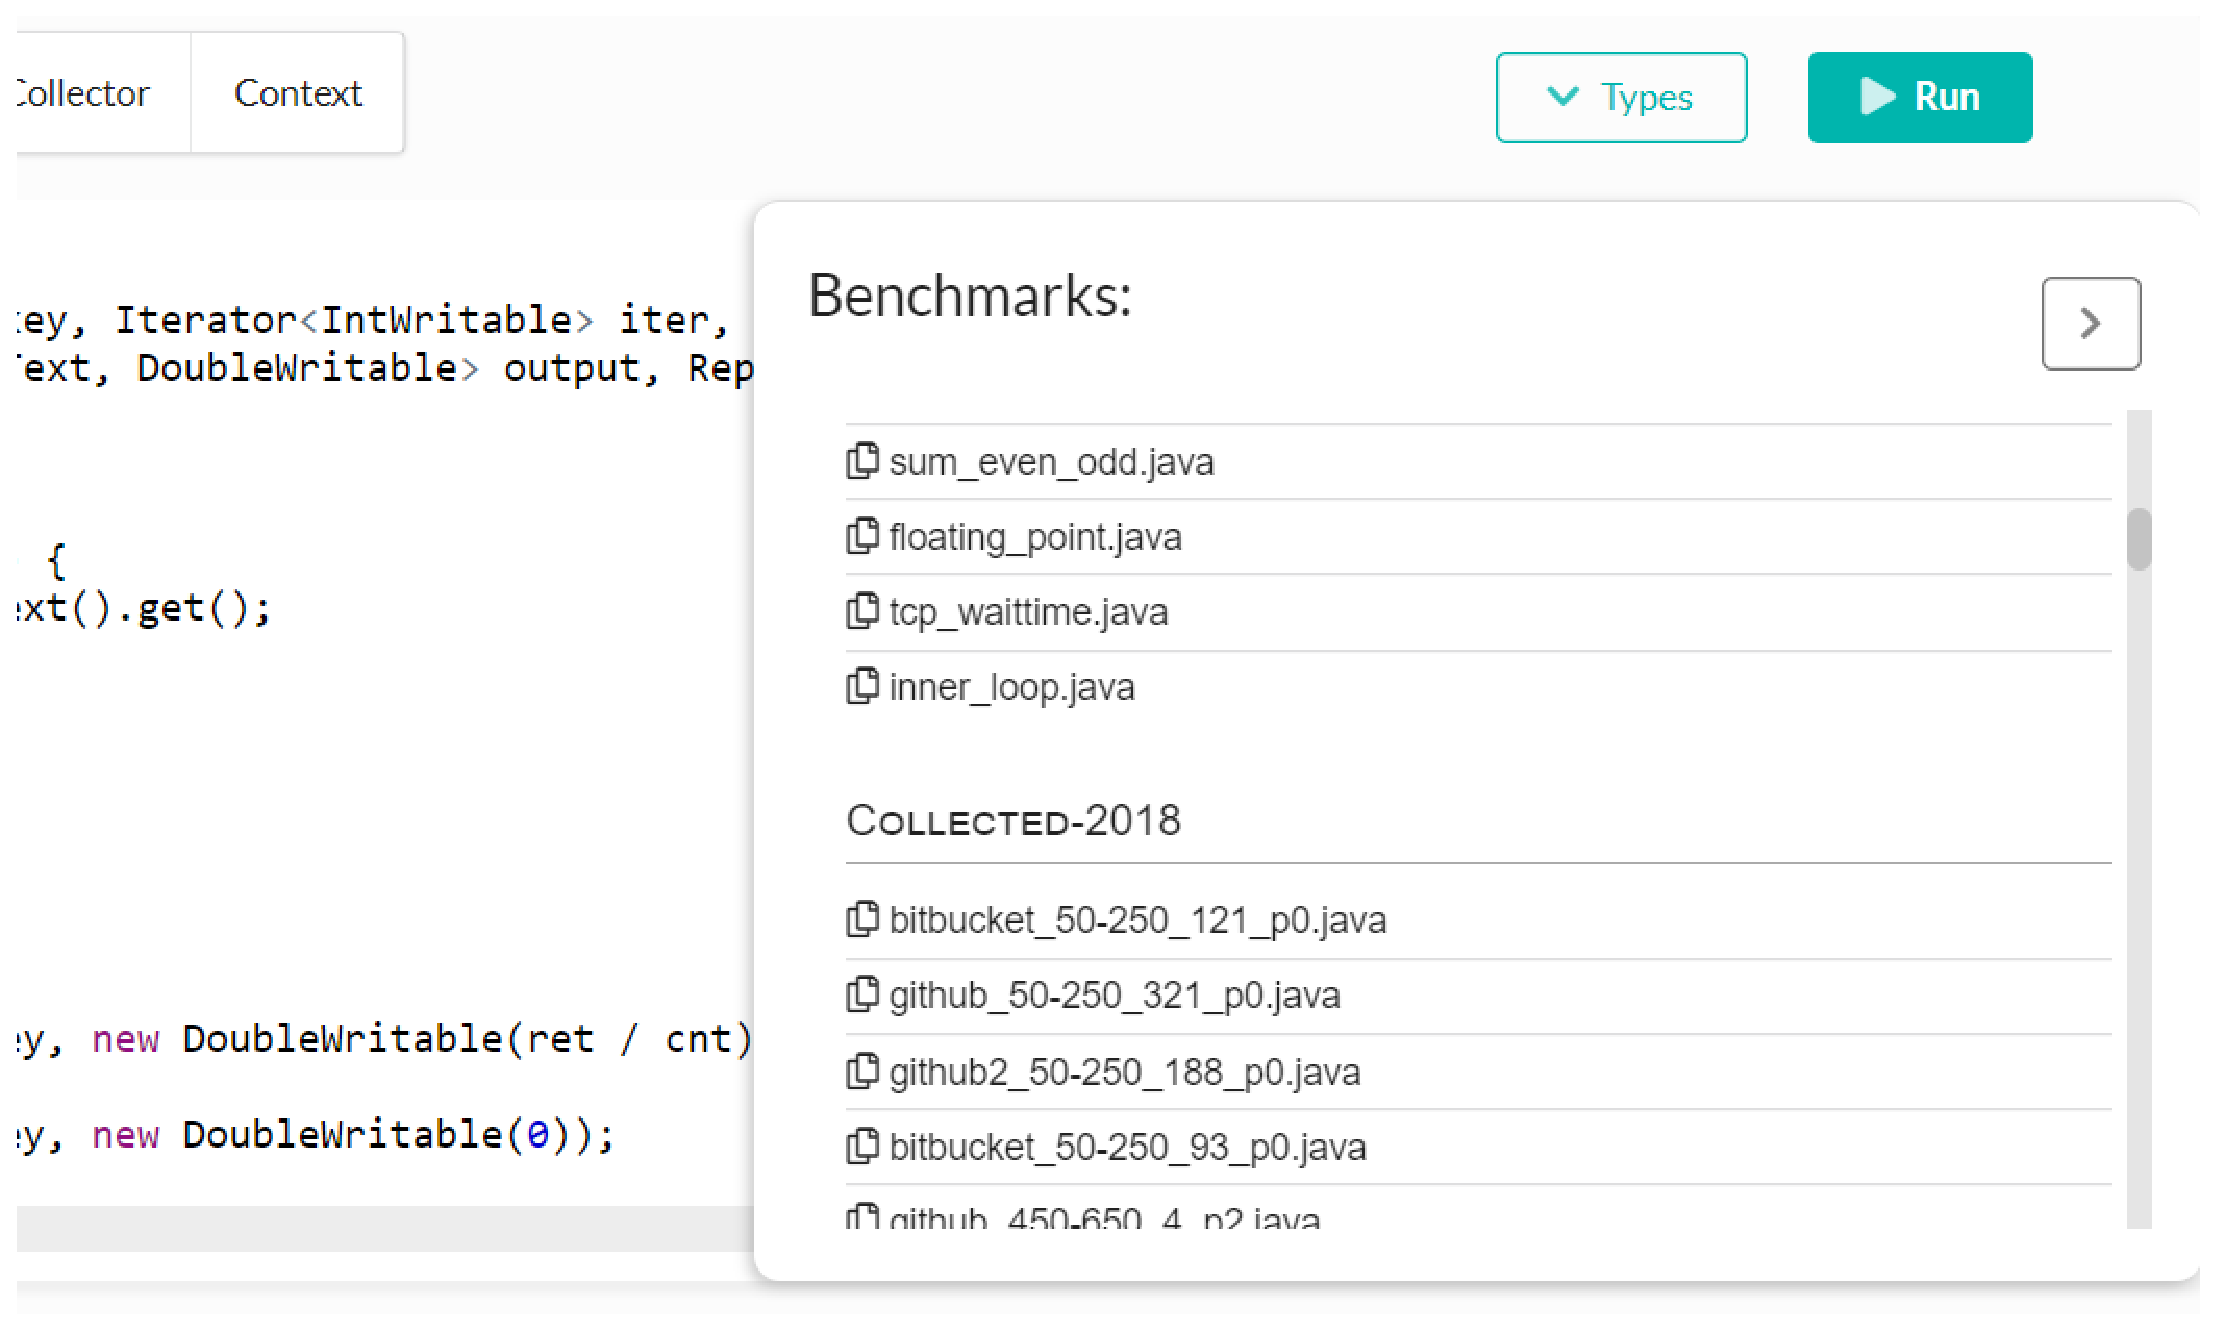
\includegraphics[width=.8\linewidth]{screenshots/benchmark_list_right}
% \vspace{-5pt}
\caption{A benchmark list from the right menu (a part).}
\label{fig:benchmark_list_right}
% \vspace{-15pt}
\end{center}
\end{figure}

\subsection{Run Analysis of a Selected Benchmark Example}
\label{appendix:2}

To run the analysis, one can choose an example from the benchmark using either
the top menu or the right menu and then click the ``Run'' button of the
upper-right menu to start the commutativity analysis of the selected example.
The pull-down menu ``Types'' of the upper-right menu provides selectable types
for input \texttt{(T1,T2)} and output \texttt{(T3,T4)} key-value pairs.
Fig.~\ref{fig:type_select_menu} shows the pull-down menu and
Fig.~\ref{fig:selectable_types} shows a part of the selectable types in
J-ReCoVer.  If one selects an example from the benchmark, the types will be
automatically selected to match the example. The selection will be needed if the
user wants to write a reduce function for analysis  from scratch (see
Appendix~\ref{appendix:3}).

\begin{figure}
\begin{center}
% \vspace{-10pt}
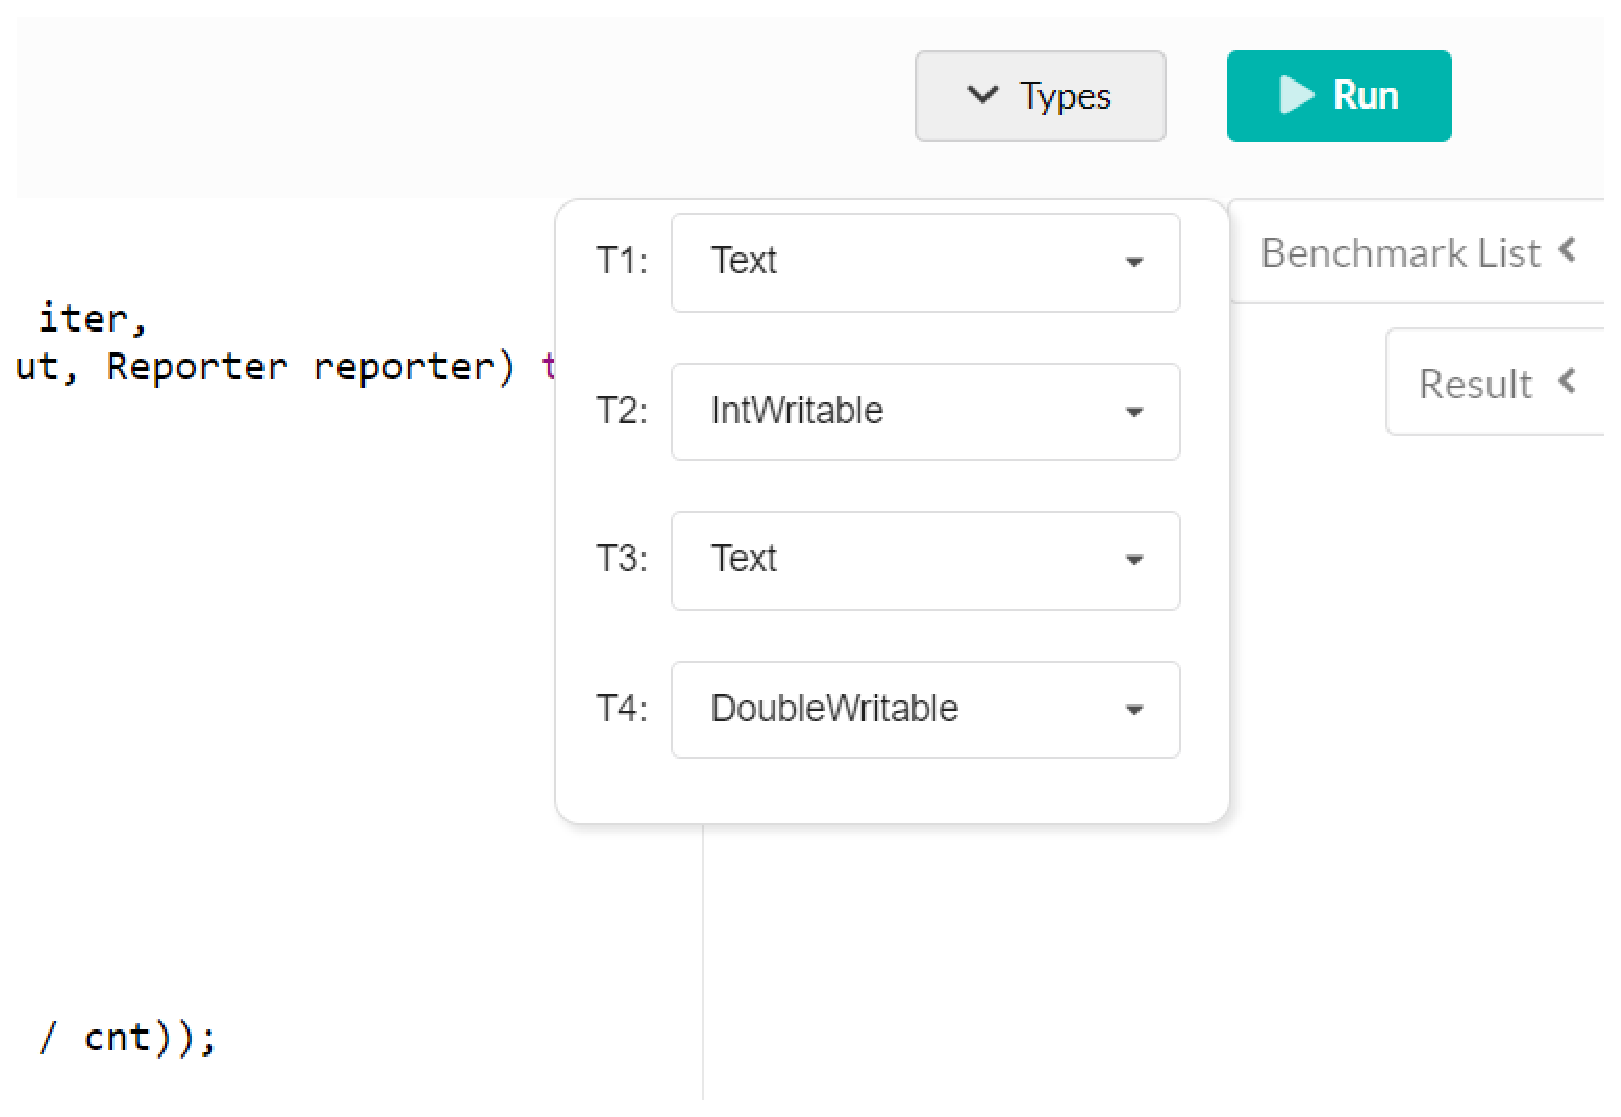
\includegraphics[width=.8\linewidth]{screenshots/type_select_menu}
% \vspace{-5pt}
\caption{The type selection menu.}
\label{fig:type_select_menu}
% \vspace{-15pt}
\end{center}
\end{figure}

\begin{figure}
\begin{center}
% \vspace{-10pt}
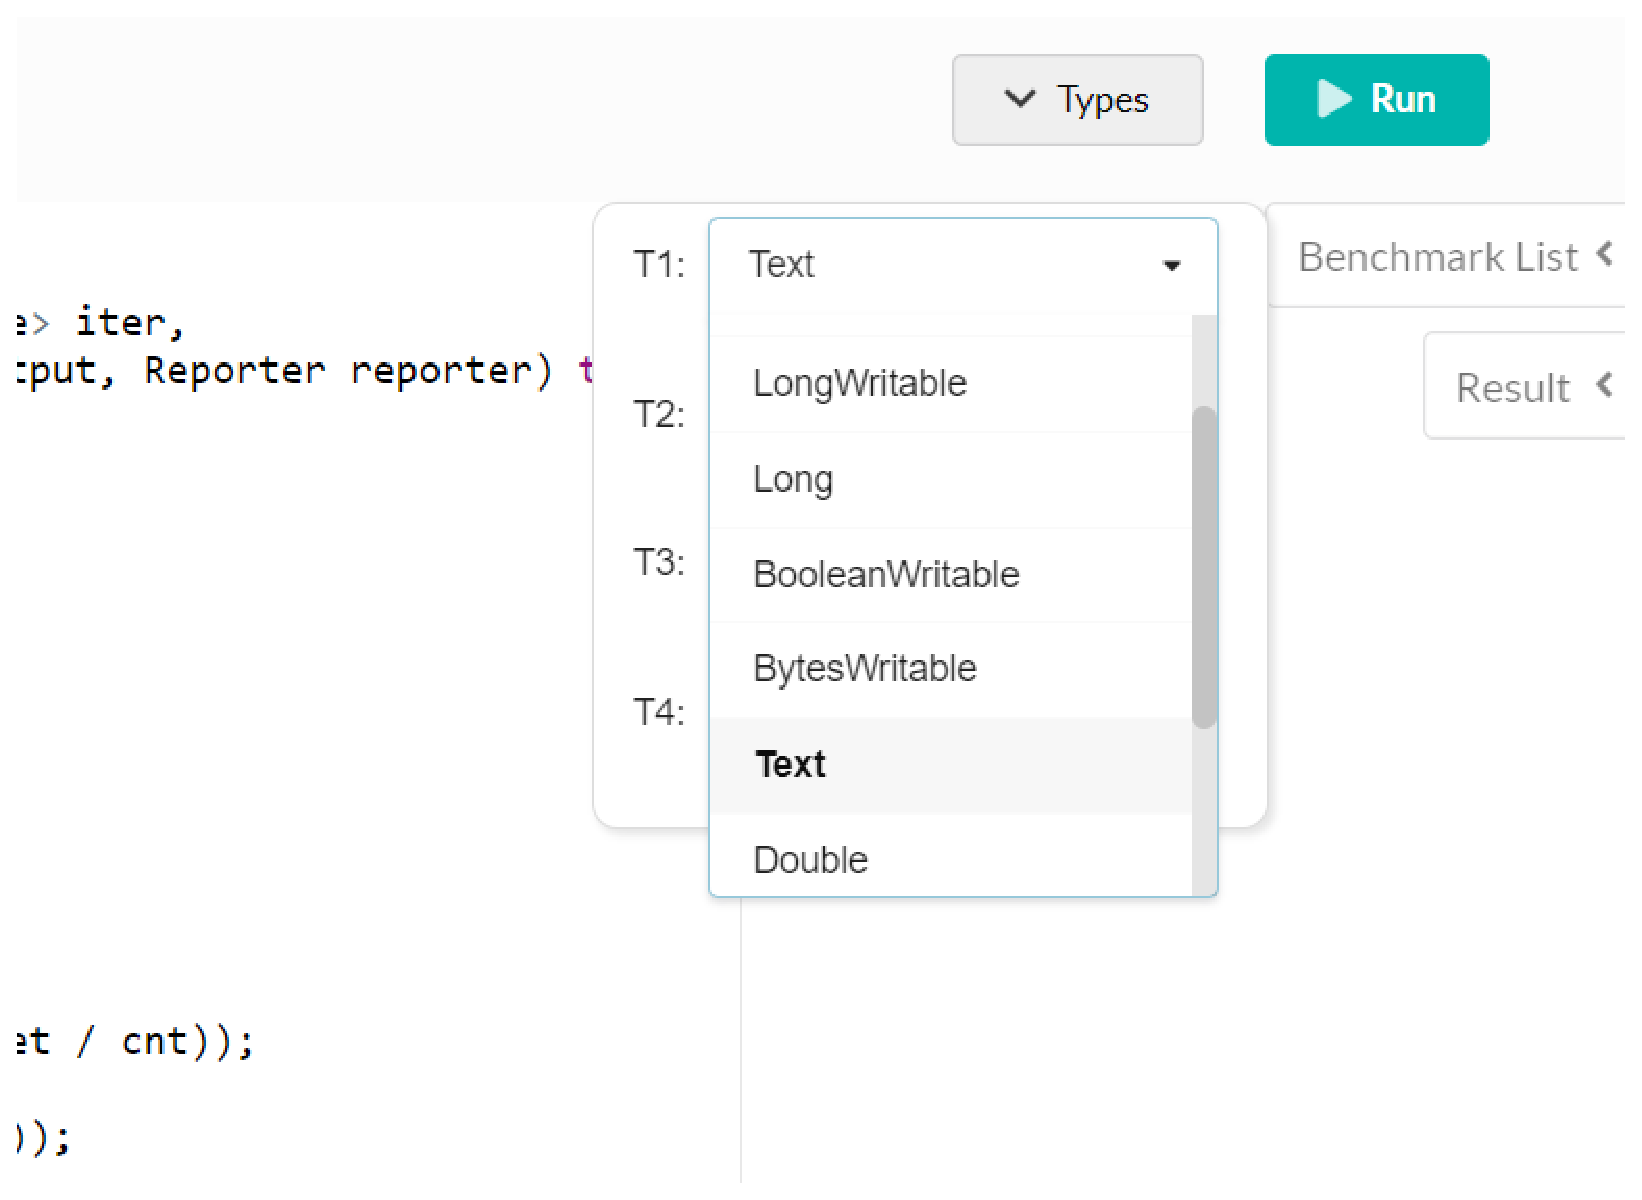
\includegraphics[width=.8\linewidth]{screenshots/selectable_types}
% \vspace{-5pt}
\caption{Selectable types (a part).}
\label{fig:selectable_types}
% \vspace{-15pt}
\end{center}
\end{figure}

After J-ReCoVer finishes the analysis, the \emph{``Result:''} tab of the right
menu will show the result of the analysis, which can be found in
Figure~\ref{fig:analysis_result}. Figure~\ref{fig:analysis_result_text} shows
the complete analysis report of the benchmark \texttt{dis.java} in
Figure~\ref{fig:main_screen}.

\begin{figure}
\begin{center}
% \vspace{-10pt}
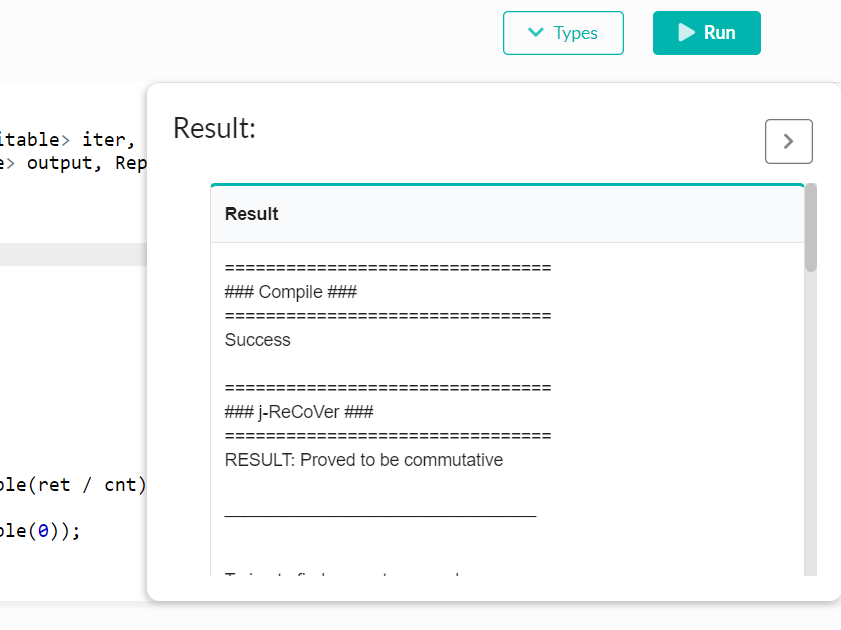
\includegraphics[width=.8\linewidth]{screenshots/analysis_result}
% \vspace{-5pt}
\caption{The analysis result.}
\label{fig:analysis_result}
% \vspace{-15pt}
\end{center}
\end{figure}

\begin{figure}
\begin{center}
\begin{mdframed}[roundcorner=5pt]
\begin{Verbatim}[fontsize=\tiny]
================================
### Compile ###
================================
Success

================================
### j-ReCoVer ###
================================
RESULT: Proved to be commutative

________________________________


Trying to find a counterexample...

RESULT: Cannot find a counterexample in 500 tests
Testcases were generated randomly.

Following are the first 50 lines of testcases:
Input1: o [5, 4, 5, 2, -1]
Input2: o [-1, 4, 5, 5, 2]
Output1: 

Key: [o]
Val: [0.0]
--
Output2: 

Key: [o]
Val: [0.0]
--------
Input1: j [1, -1, 0, 3, -2]
Input2: j [0, 3, -2, 1, -1]
Output1: 

Key: [j]
Val: [0.0]
--
Output2: 

Key: [j]
Val: [0.0]
--------
Input1: e [4, 3, 5, -4, 1]
Input2: e [4, -4, 5, 3, 1]
Output1: 

Key: [e]
Val: [0.0]
--
Output2: 

Key: [e]
Val: [0.0]
--------
Input1: s [3, 0, 2, -4, -1]
Input2: s [3, -1, 0, -4, 2]
Output1: 

Key: [s]
Val: [0.0]
--
Output2: 

Key: [s]
Val: [0.0]
--------
Input1: v [-3, -2, 3, 3, -3]
Input2: v [3, -2, -3, -3, 3]
\end{Verbatim}
\end{mdframed}
\caption{The analysis result of \texttt{dis.java}.}
\label{fig:analysis_result_text}
\end{center}
\end{figure}

When an analysis is started, J-ReCoVer first tries to compile the chosen example
and then performs its commutativity analysis. If the analysis cannot conclude
that the example is commutative, J-ReCoVer then runs 500 randomly generated test
cases to try to find a counterexample. If the test cases all pass, then the
result will be ``unknown''.

\clearpage
\subsection{Run Analysis of a User-defined Reducer Function}
\label{appendix:3}

Besides examples from the benchmark, J-ReCoVer also provides an interactive way
for analysing a user-defined reducer function.  One can directly edit the code
of a selected example in the coding space for further analysis, or write a
reducer function from scratch. The upper-left menu (below the top menu)
provides blank templates for two versions of Hadoop. The templates are shown
below:

\begin{mdframed}[roundcorner=5pt]
\begin{verbatim}
public void reduce(T1 key, Iterator<T2> values,
	OutputCollector<T3,T4> oc1, Reporter reporter)
		throws IOException,InterruptedException {

}
\end{verbatim}
\end{mdframed}

\begin{mdframed}[roundcorner=5pt]
\begin{verbatim}
public void reduce(T1 key, Iterable<T2> values,
	Context context) throws IOException,InterruptedException {

}
\end{verbatim}
\end{mdframed}

In this case, one would have to manually fill the types T1 to T4 and the
function body, and then select the types from the pull-down menu as shown in
Figure~\ref{fig:type_select_menu} and Figure~\ref{fig:selectable_types}. All
selectable types are:

\begin{itemize}
\item Long,
\item BooleanWritable,
\item BytesWritable,
\item Text,
\item Double,
\item DoubleWritable,
\item Float,
\item FloatWritable.
\end{itemize}
